\documentclass[11pt,a4paper]{article}

\usepackage[margin=1in]{geometry}
\usepackage{graphicx}
\usepackage{float}
\usepackage{amsmath}
\usepackage[utf8]{inputenc}
\usepackage[T1]{fontenc}
\usepackage{lmodern}
\usepackage{microtype}
\usepackage{csquotes}
\usepackage[english]{babel}
\usepackage{cite}
\usepackage{listings}
\usepackage{xcolor}
\usepackage{caption,subcaption}
\usepackage{booktabs}
\usepackage[hidelinks]{hyperref}

\lstset{
    basicstyle=\ttfamily\small,
    keywordstyle=\color{blue},
    commentstyle=\color{gray},
    breaklines=true
}
 
\makeatletter
% allow a subtitle
\providecommand\@subtitle{}
\newcommand{\subtitle}[1]{\gdef\@subtitle{#1}}

% provide a way to set two author emails
\providecommand\@emailone{email1@example.com}
\providecommand\@emailtwo{email2@example.com}
\newcommand{\authoremails}[2]{\gdef\@emailone{#1}\gdef\@emailtwo{#2}}

% default subtitle and emails (editable)
\subtitle{Máster en Inteligencia Artificial - Universidad de Murcia}
\authoremails{jdiego.gallego@um.es}{oscar.veral@um.es}

% Redefine \maketitle to produce a dedicated titlepage
\renewcommand{\maketitle}{%
    \begin{titlepage}
        \centering
        \thispagestyle{empty}
        \vspace*{2.5cm}
        {\Huge\bfseries\@title\par}
        \vspace{1cm}
        {\Large\itshape\@subtitle\par}
        \vspace{3cm}
        {\large
            \begin{tabular}{c}
                \@author
            \end{tabular}\par
        }
        \vspace{0.6cm}
        {\small
            \begin{tabular}{c}
                \texttt{\@emailone} \\[0.8ex]
                \texttt{\@emailtwo}
            \end{tabular}\par
        }
        \vfill
        {\large \@date\par}
    \end{titlepage}%
}
\makeatother

\begin{document}

\title{BT4\\[1ex]\large Visión Artificial}
\author{Juan Diego Gallego Nicolás \and Óscar Vera López}
\date{\today}

\maketitle

\renewcommand{\contentsname}{Índice}
\setcounter{tocdepth}{3}
\tableofcontents
\clearpage

\section*{Introducción}
En este informe se detallan las implementaciones y resultados obtenidos en las tareas de procesamiento de imágenes realizadas en el contexto de los bloques de trabajo BT4.
Cada bloque de técnicas recibe su propio apartado. 
Todas las referencias a código fuente, notebooks y datos se encuentran en el repositorio de GitHub asociado al proyecto: \href{https://github.com/oscarveral/vision}{vision}

\section*{Items cubiertos}
\begin{itemize}
  \item \textbf{TODO}.
\end{itemize}


\clearpage
\section{BT4 - Deep Learning para visión por computador}

Para las aplicaciones de Deep Learning hemos querido centrarnos en la detección de objetos. En el caso de nuestro dataset,
buscamos detecctar señales de tráfico. Para esta tarea, hemos escogido reentrenar modelos de la familia YOLOv8.

\textit{Items de evaluación: \underline{\textbf{BT1h}},
\underline{\textbf{BT1ewc}}.}

\subsection{Arquitectura del modelo}

Para la detección de las señales, hemos seleccionado la arquitectura \textbf{YOLOv8} 
(You Only Look Once, versión 8), desarrollada por Ultralytics. 
Este modelo pertenece a la familia de detectores de una sola etapa (\textit{one-stage detectors}), 
lo que significa que realiza la predicción de las cajas delimitadoras y las probabilidades de clase en 
una única pasada por la red neuronal, optimizando el equilibrio entre velocidad de inferencia y precisión.

La arquitectura YOLOv8 se basa en una combinación de bloques convolucionales que se organizan en tres etapas:

\begin{itemize}
    \item \textbf{Backbone:} Esta etapa inicial extrae características de bajo nivel de las imágenes de entrada mediante 
            una serie de capas convolucionales y bloques residuales. Utiliza técnicas como la normalización por lotes 
            y funciones de activación no lineales para mejorar la capacidad de representación.
    
    \item \textbf{Neck:} La segunda etapa, conocida como \textit{neck}, agrega y fusiona las características extraídas por el 
            \textit{backbone} a través de estructuras como PANet (Path Aggregation Network). Esto permite al modelo 
            capturar información a múltiples escalas, esencial para detectar objetos de diferentes tamaños.

    \item \textbf{Head:} La etapa final, el \textit{head}, es responsable de generar las predicciones finales. 
            Utiliza capas convolucionales para predecir las cajas delimitadoras, las puntuaciones de confianza y 
            las probabilidades de clase para cada objeto detectado.
\end{itemize}

\subsection{Preparación de datos}

YOLOv8 requiere que los datos estén en un formato específico donde cada imagen debe ir acompañada de un archivo de texto (\texttt{.txt}) 
con el mismo nombre, donde cada línea representa un objeto detectado en el formato normalizado:
\[ \text{<clase>} \ \text{<x\_centro>} \ \text{<y\_centro>} \ \text{<ancho>} \ \text{<alto>} \]
donde todas las coordenadas están normalizadas entre 0 y 1 respecto a las dimensiones de la imagen.
Además, durante las primeras iteraciones experimentales, detectamos que el uso directo de las anotaciones originales impedía la correcta convergencia del modelo 
debido a dos factores críticos: la presencia de coordenadas erróneas (valores negativos o fuera de los límites de la imagen) y la existencia 
de señales de tráfico extremadamente pequeñas (ruido) captadas a muy larga distancia.

Para solucionar estos problemas y garantizar la calidad del entrenamiento, 
implementamos un pipeline de curación de datos en Python (\texttt{zod2yolo.py}) que 
aplica las siguientes transformaciones:

\begin{itemize}
    \item \textbf{Conversión y Normalización:} Transformación de las coordenadas absolutas del 
            fichero \texttt{object\_detection.json} original a las coordenadas relativas requeridas por YOLO 
            tomando como referencia la resolución de las imágenes ($3848 \times 2168$).
    
    \item \textbf{Clamping de Coordenadas:} Aplicamos una función de recorte (\textit{clamping}) 
            para asegurar que ninguna caja (\textit{bounding box}) excediera los límites de la imagen, 
            corrigiendo valores negativos o fuera de los límites que generan errores en el cálculo de la pérdida.
            Cabe destacar que los delimitadores originales de ZOD no son rectángulos, sino polígonos de cuatro puntos.
            Así pues, para cada caja, calculamos el rectángulo mínimo que la contiene y aplicamos el clamping sobre este.
    
    \item \textbf{Filtrado por Tamaño Mínimo:} Establecemos un umbral de filtrado para descartar cualquier 
            objeto cuya área fuera inferior a $15 \times 15$ píxeles. Esta medida es necesaria
            para poder entrenar el modelo para detectar las señales de tráfico más relevantes
            para el conductor, pues estas son las que aparecen con un tamaño suficiente en la imagen.

    \item \textbf{Inclusión de Muestras Negativas:} Existen imágenes en el dataset original que no contienen señales de tráfico. 
            Estas imágenes son valiosas para el entrenamiento, ya que ayudan al modelo a aprender a distinguir entre 
            escenas con y sin señales. Por ello, incluimos estas imágenes en el dataset final, 
            generando archivos \texttt{.txt} vacíos para ellas.
\end{itemize}

El dataset resultante, denominado \texttt{bt4}, consta de un subconjunto de 2,000 imágenes 
seleccionadas de forma uniformemente aleatoria de entre las primeras 50,000 de ZOD. 
Estas se encuentran divididas en un 80\% para entrenamiento (\textit{Train}) y un 20\% 
para validación (\textit{Val}) acompañadas de sus correspondientes archivos de anotaciones en formato YOLO.

% Un mosaico 3x2 de imágenes de ejemplo con sus bounding boxes
\begin{figure}[H]
    \centering
    \begin{tabular}{ccc}
        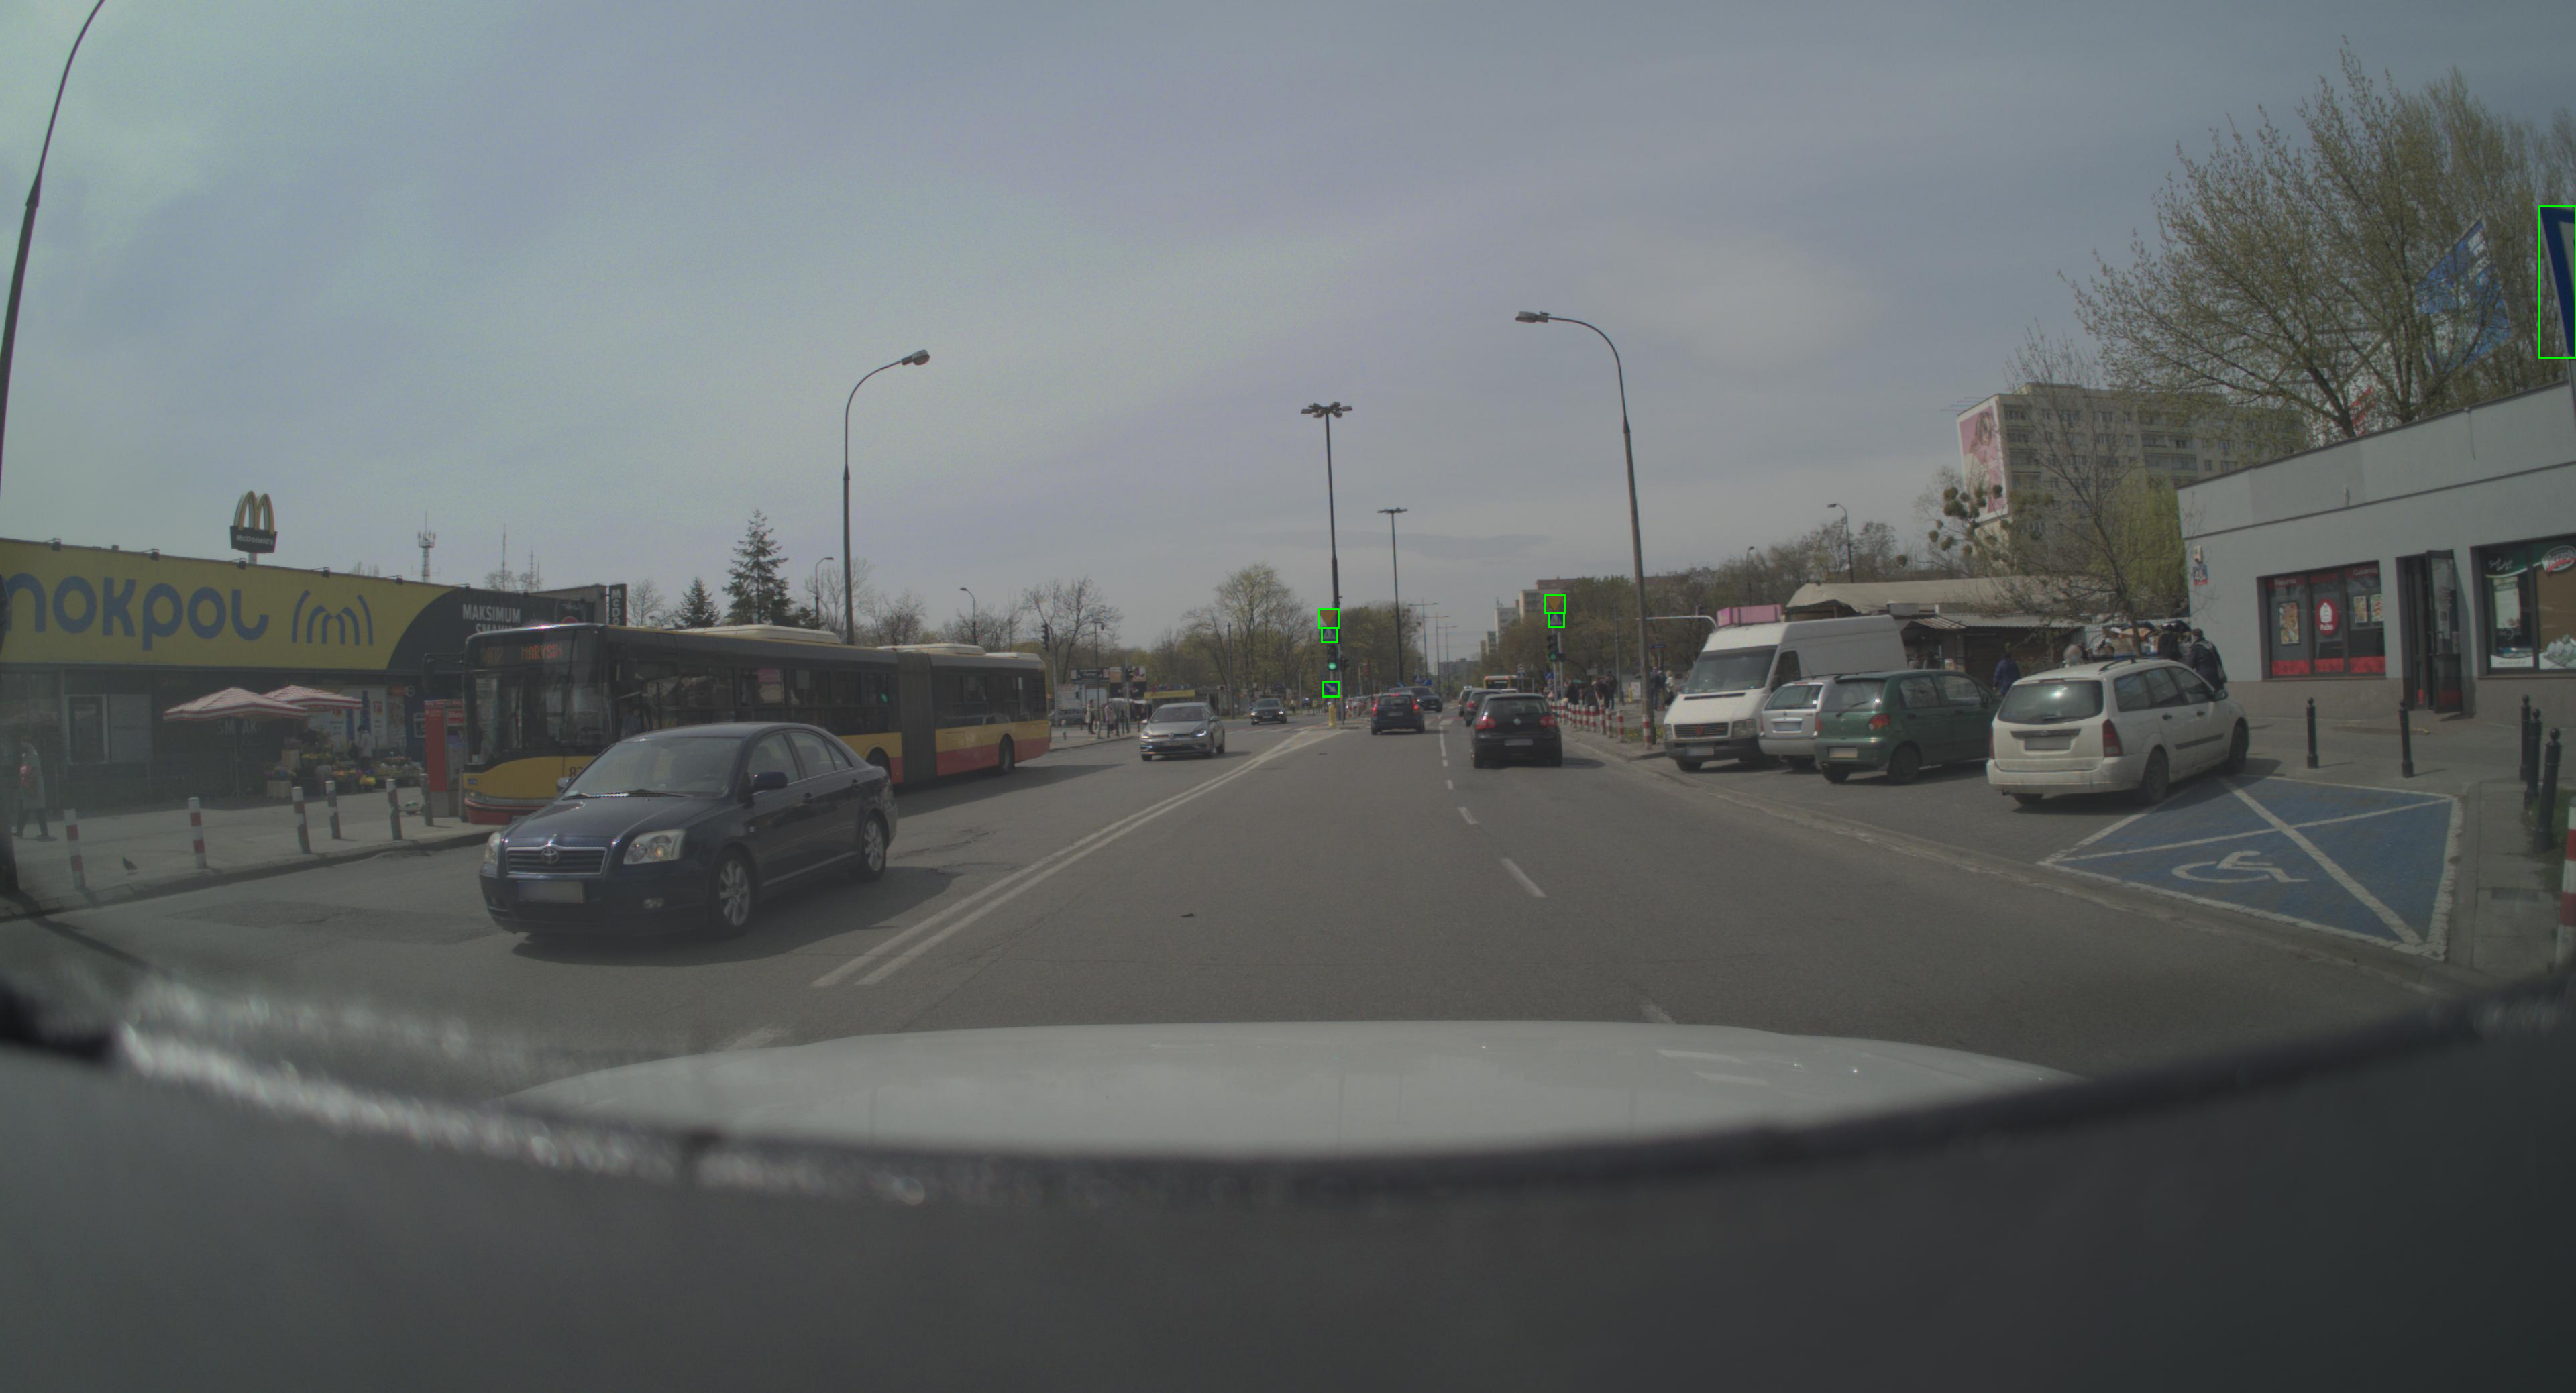
\includegraphics[width=0.49\textwidth]{images/bt4/000080.png} &
        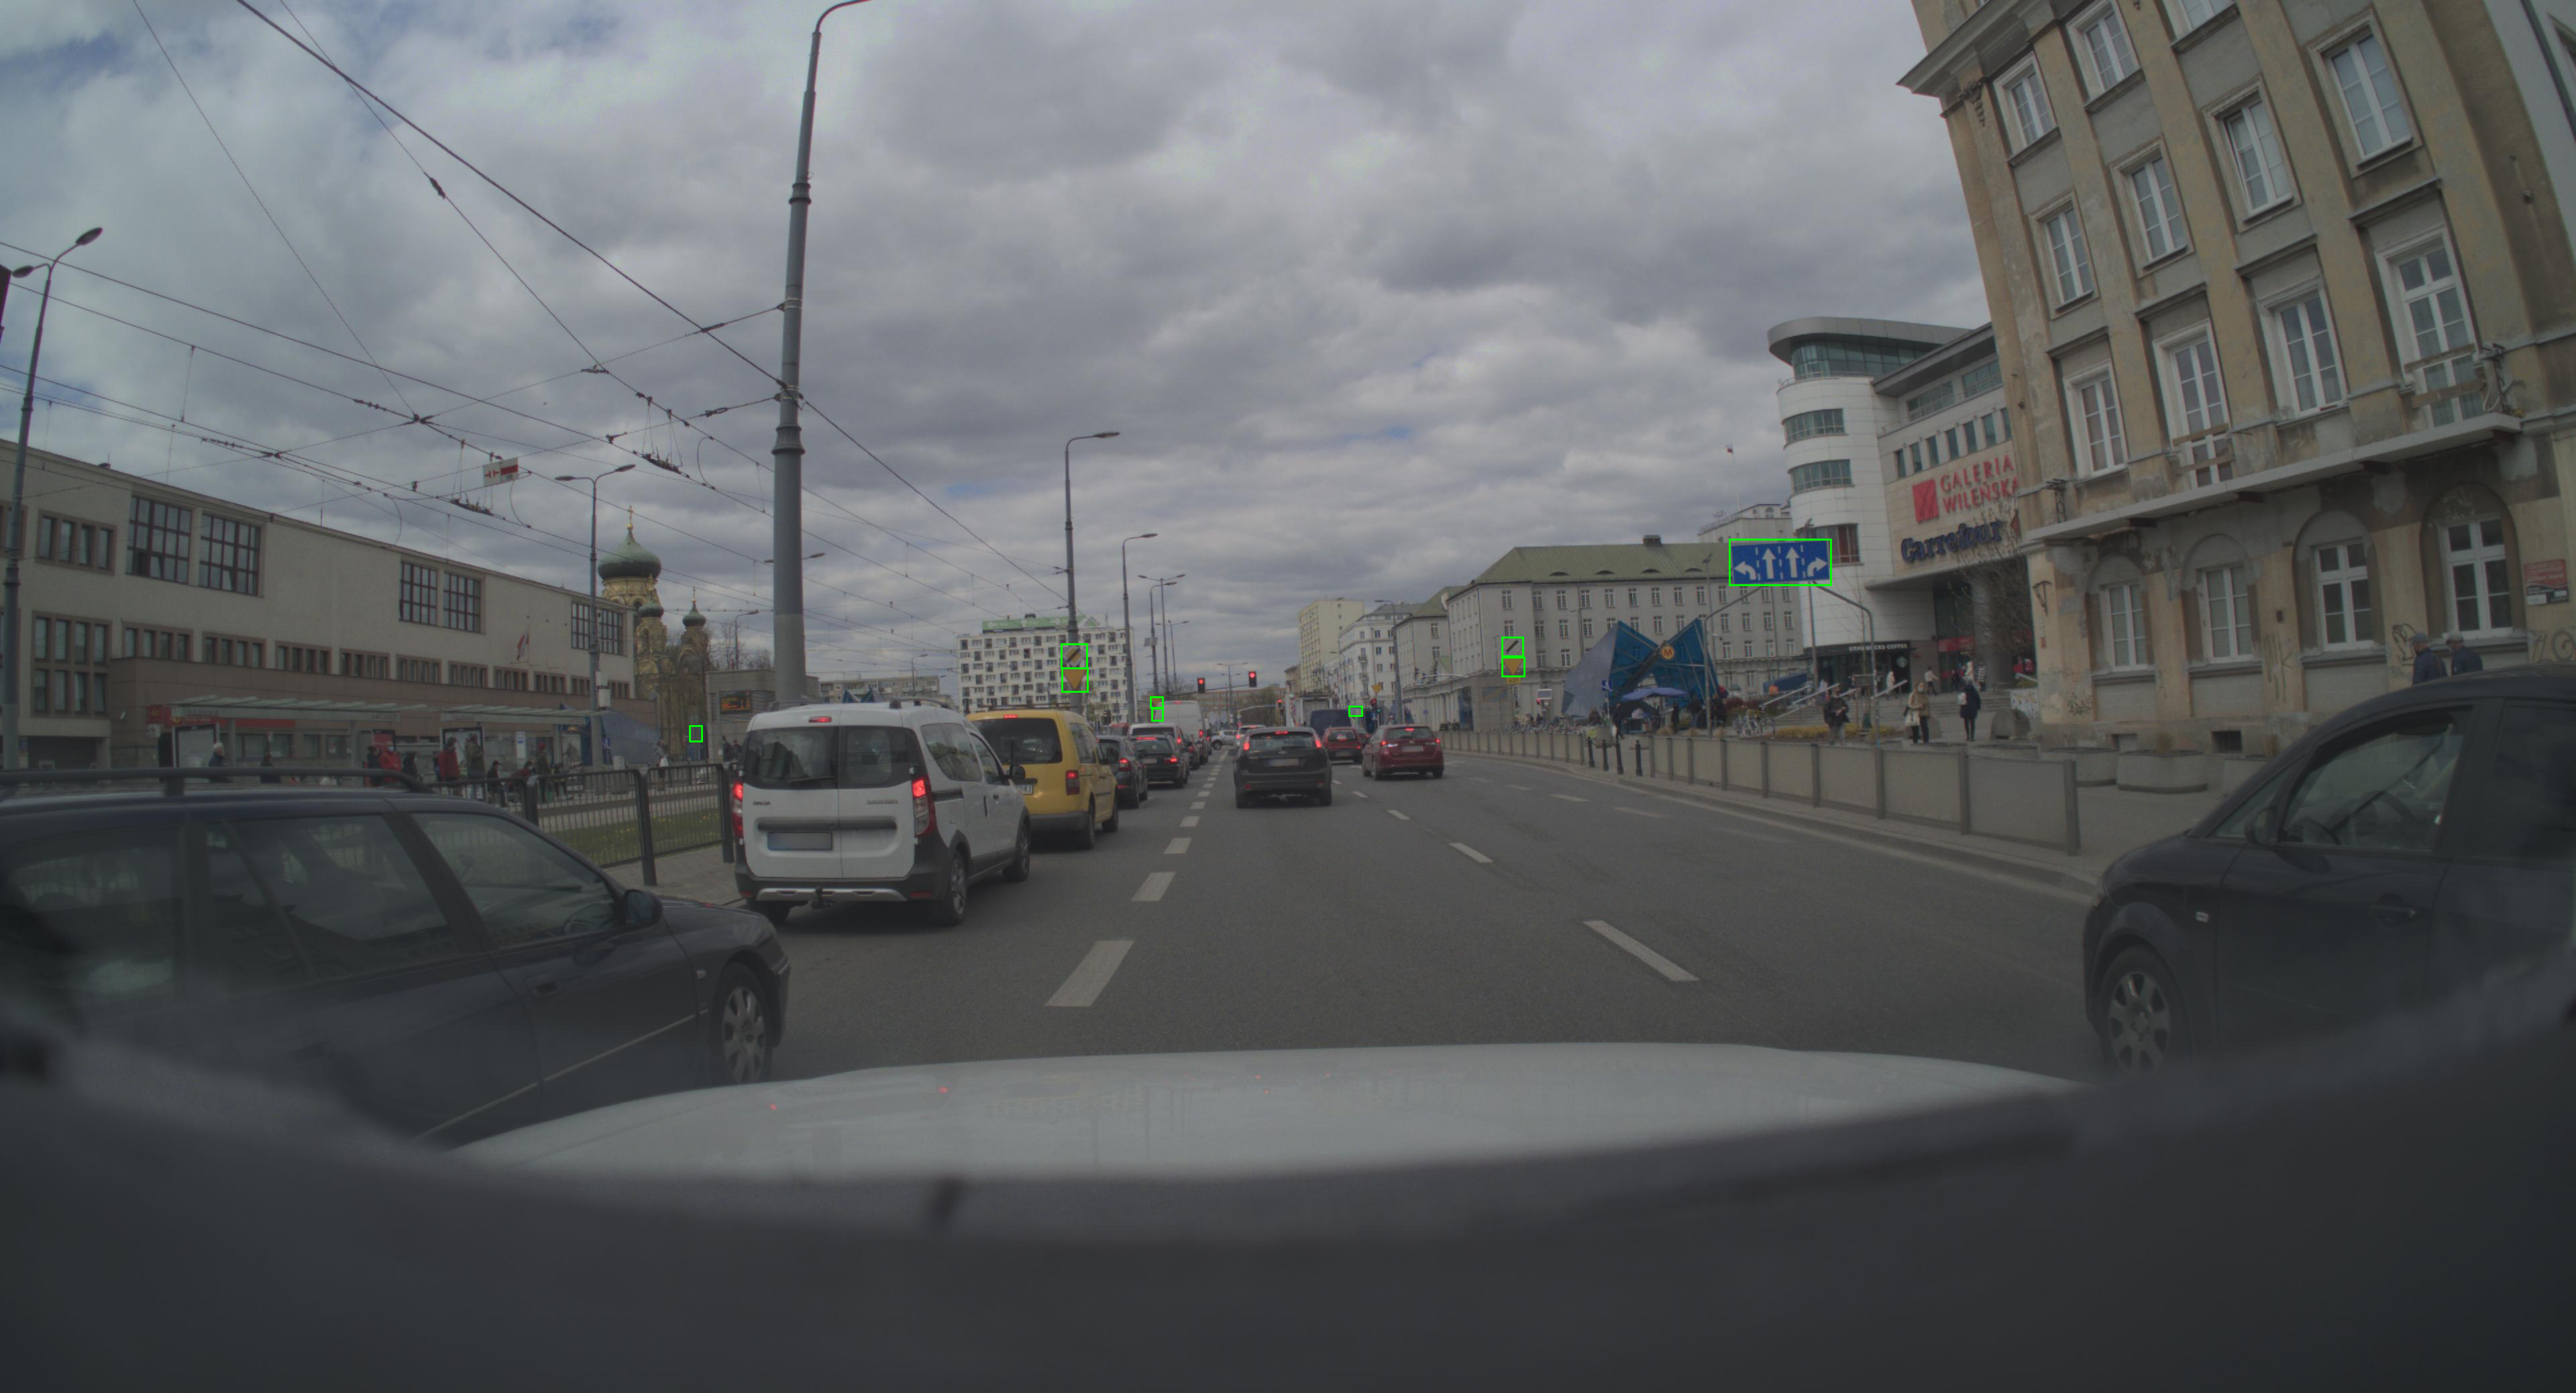
\includegraphics[width=0.49\textwidth]{images/bt4/000196.png} \\
        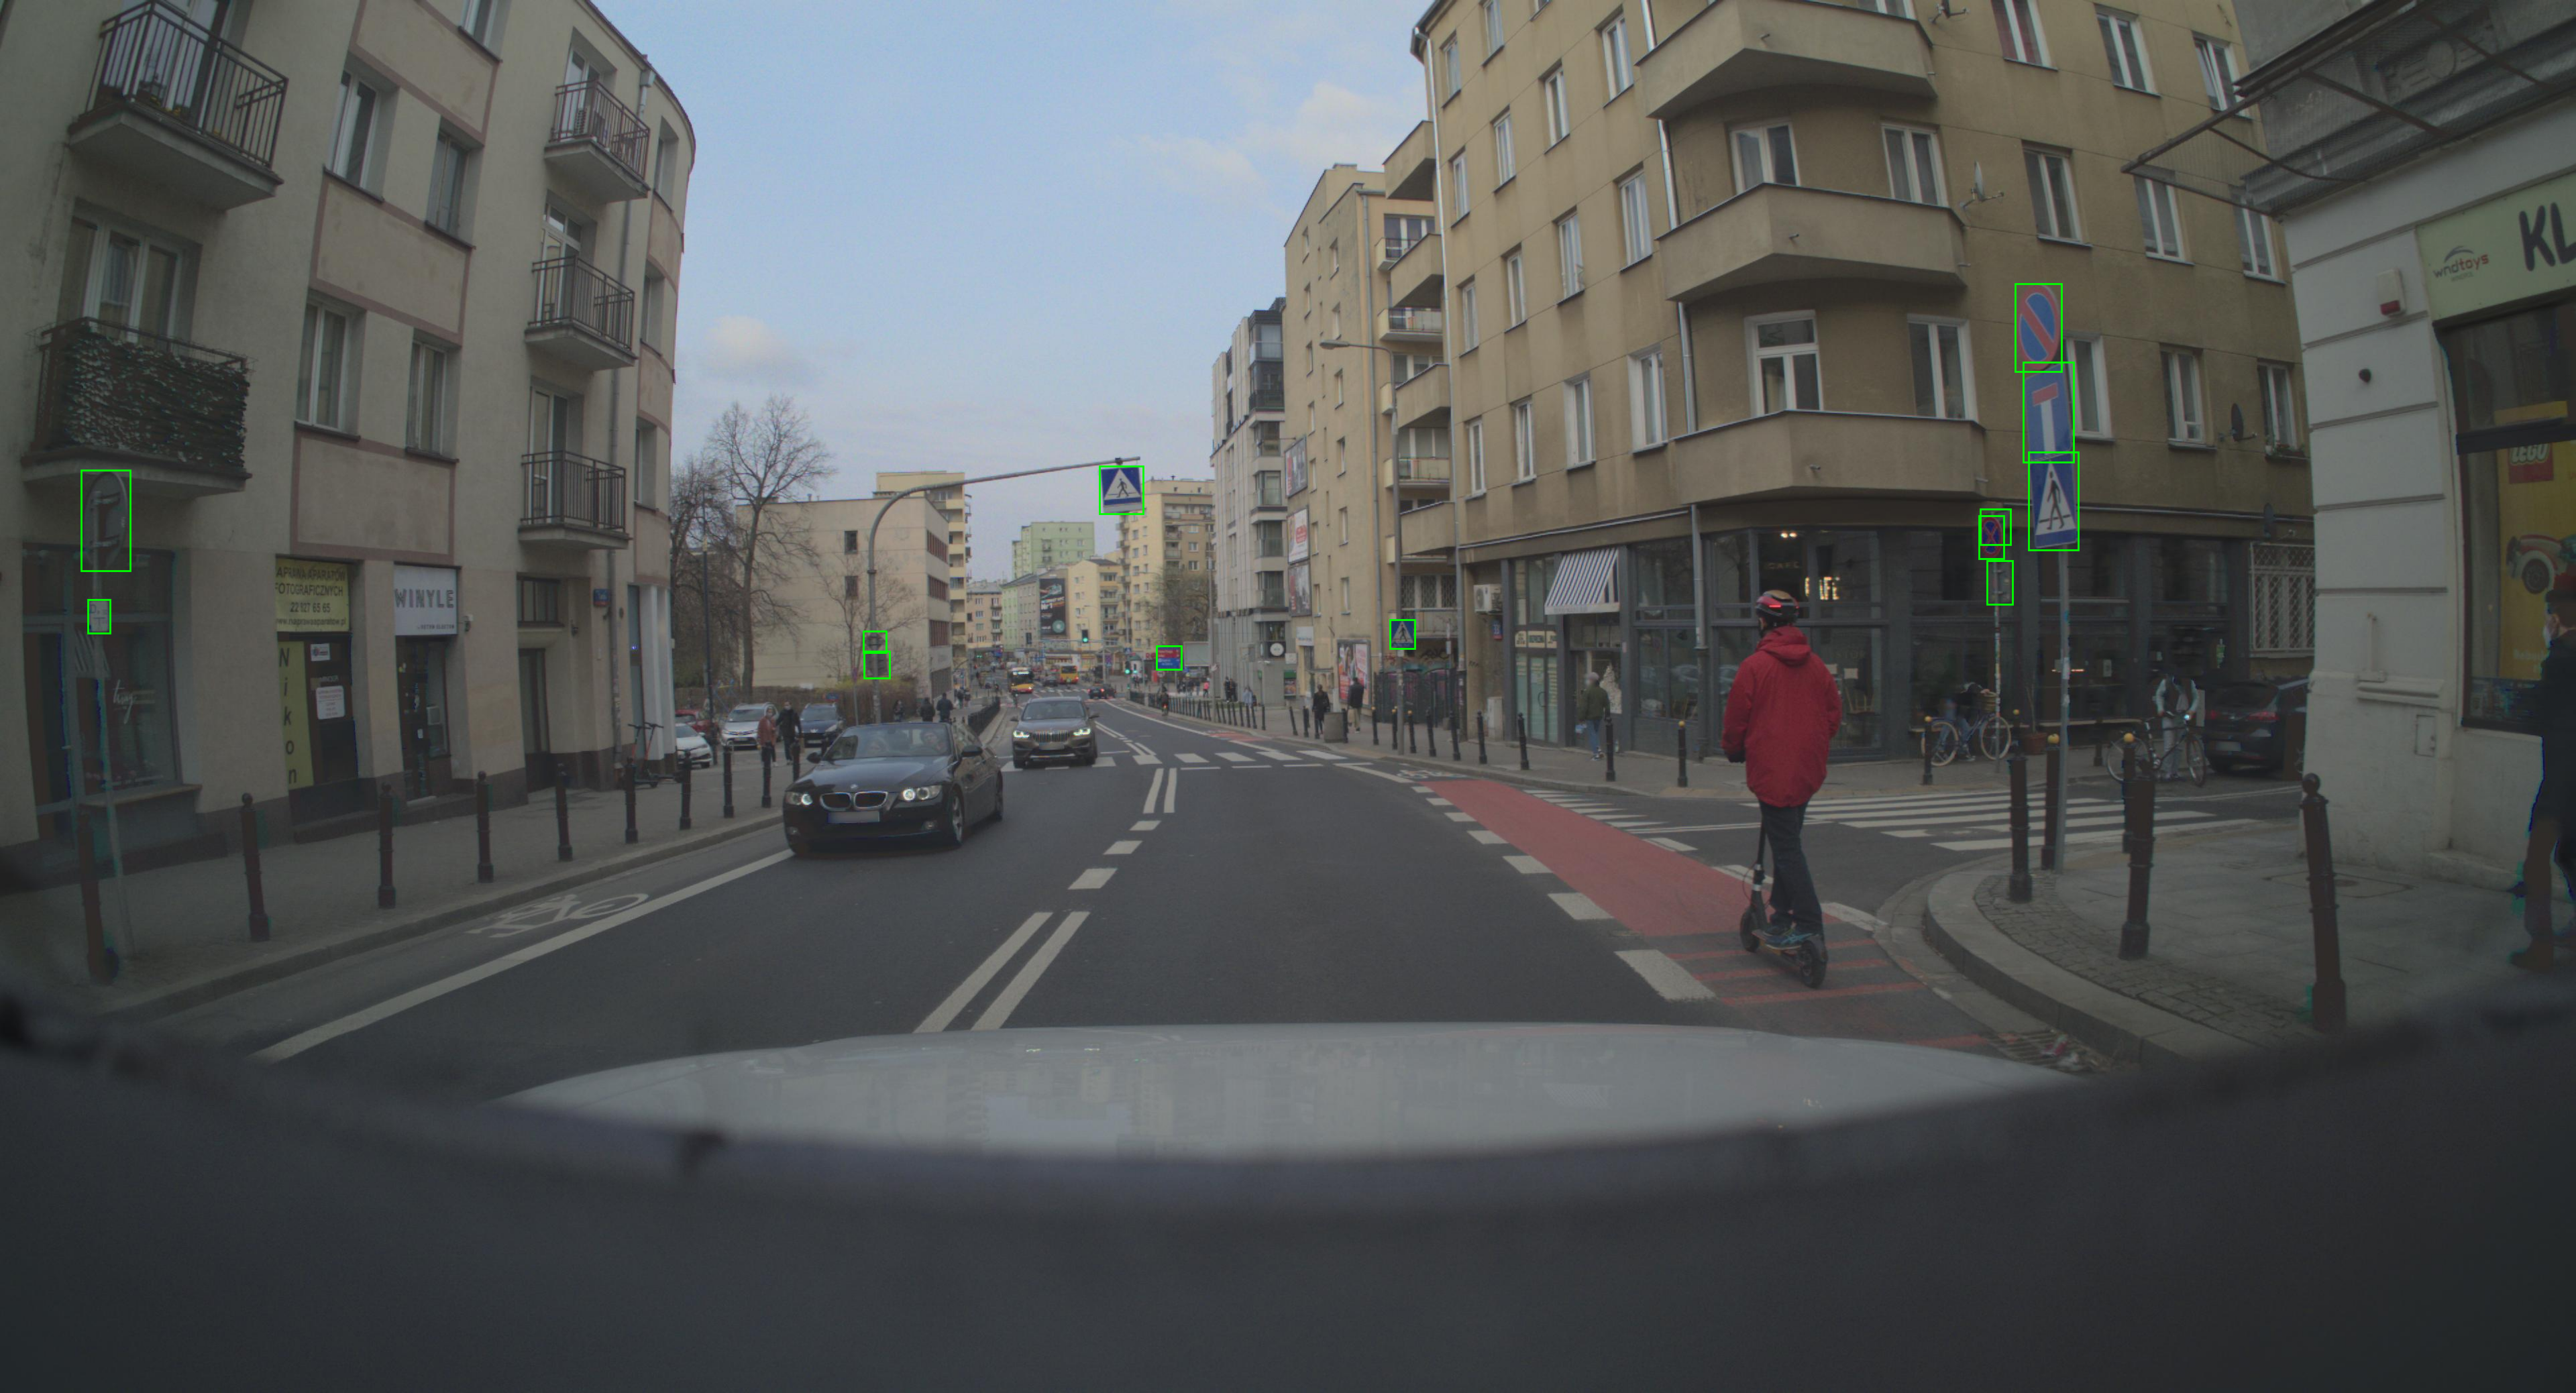
\includegraphics[width=0.49\textwidth]{images/bt4/000329.png} &
        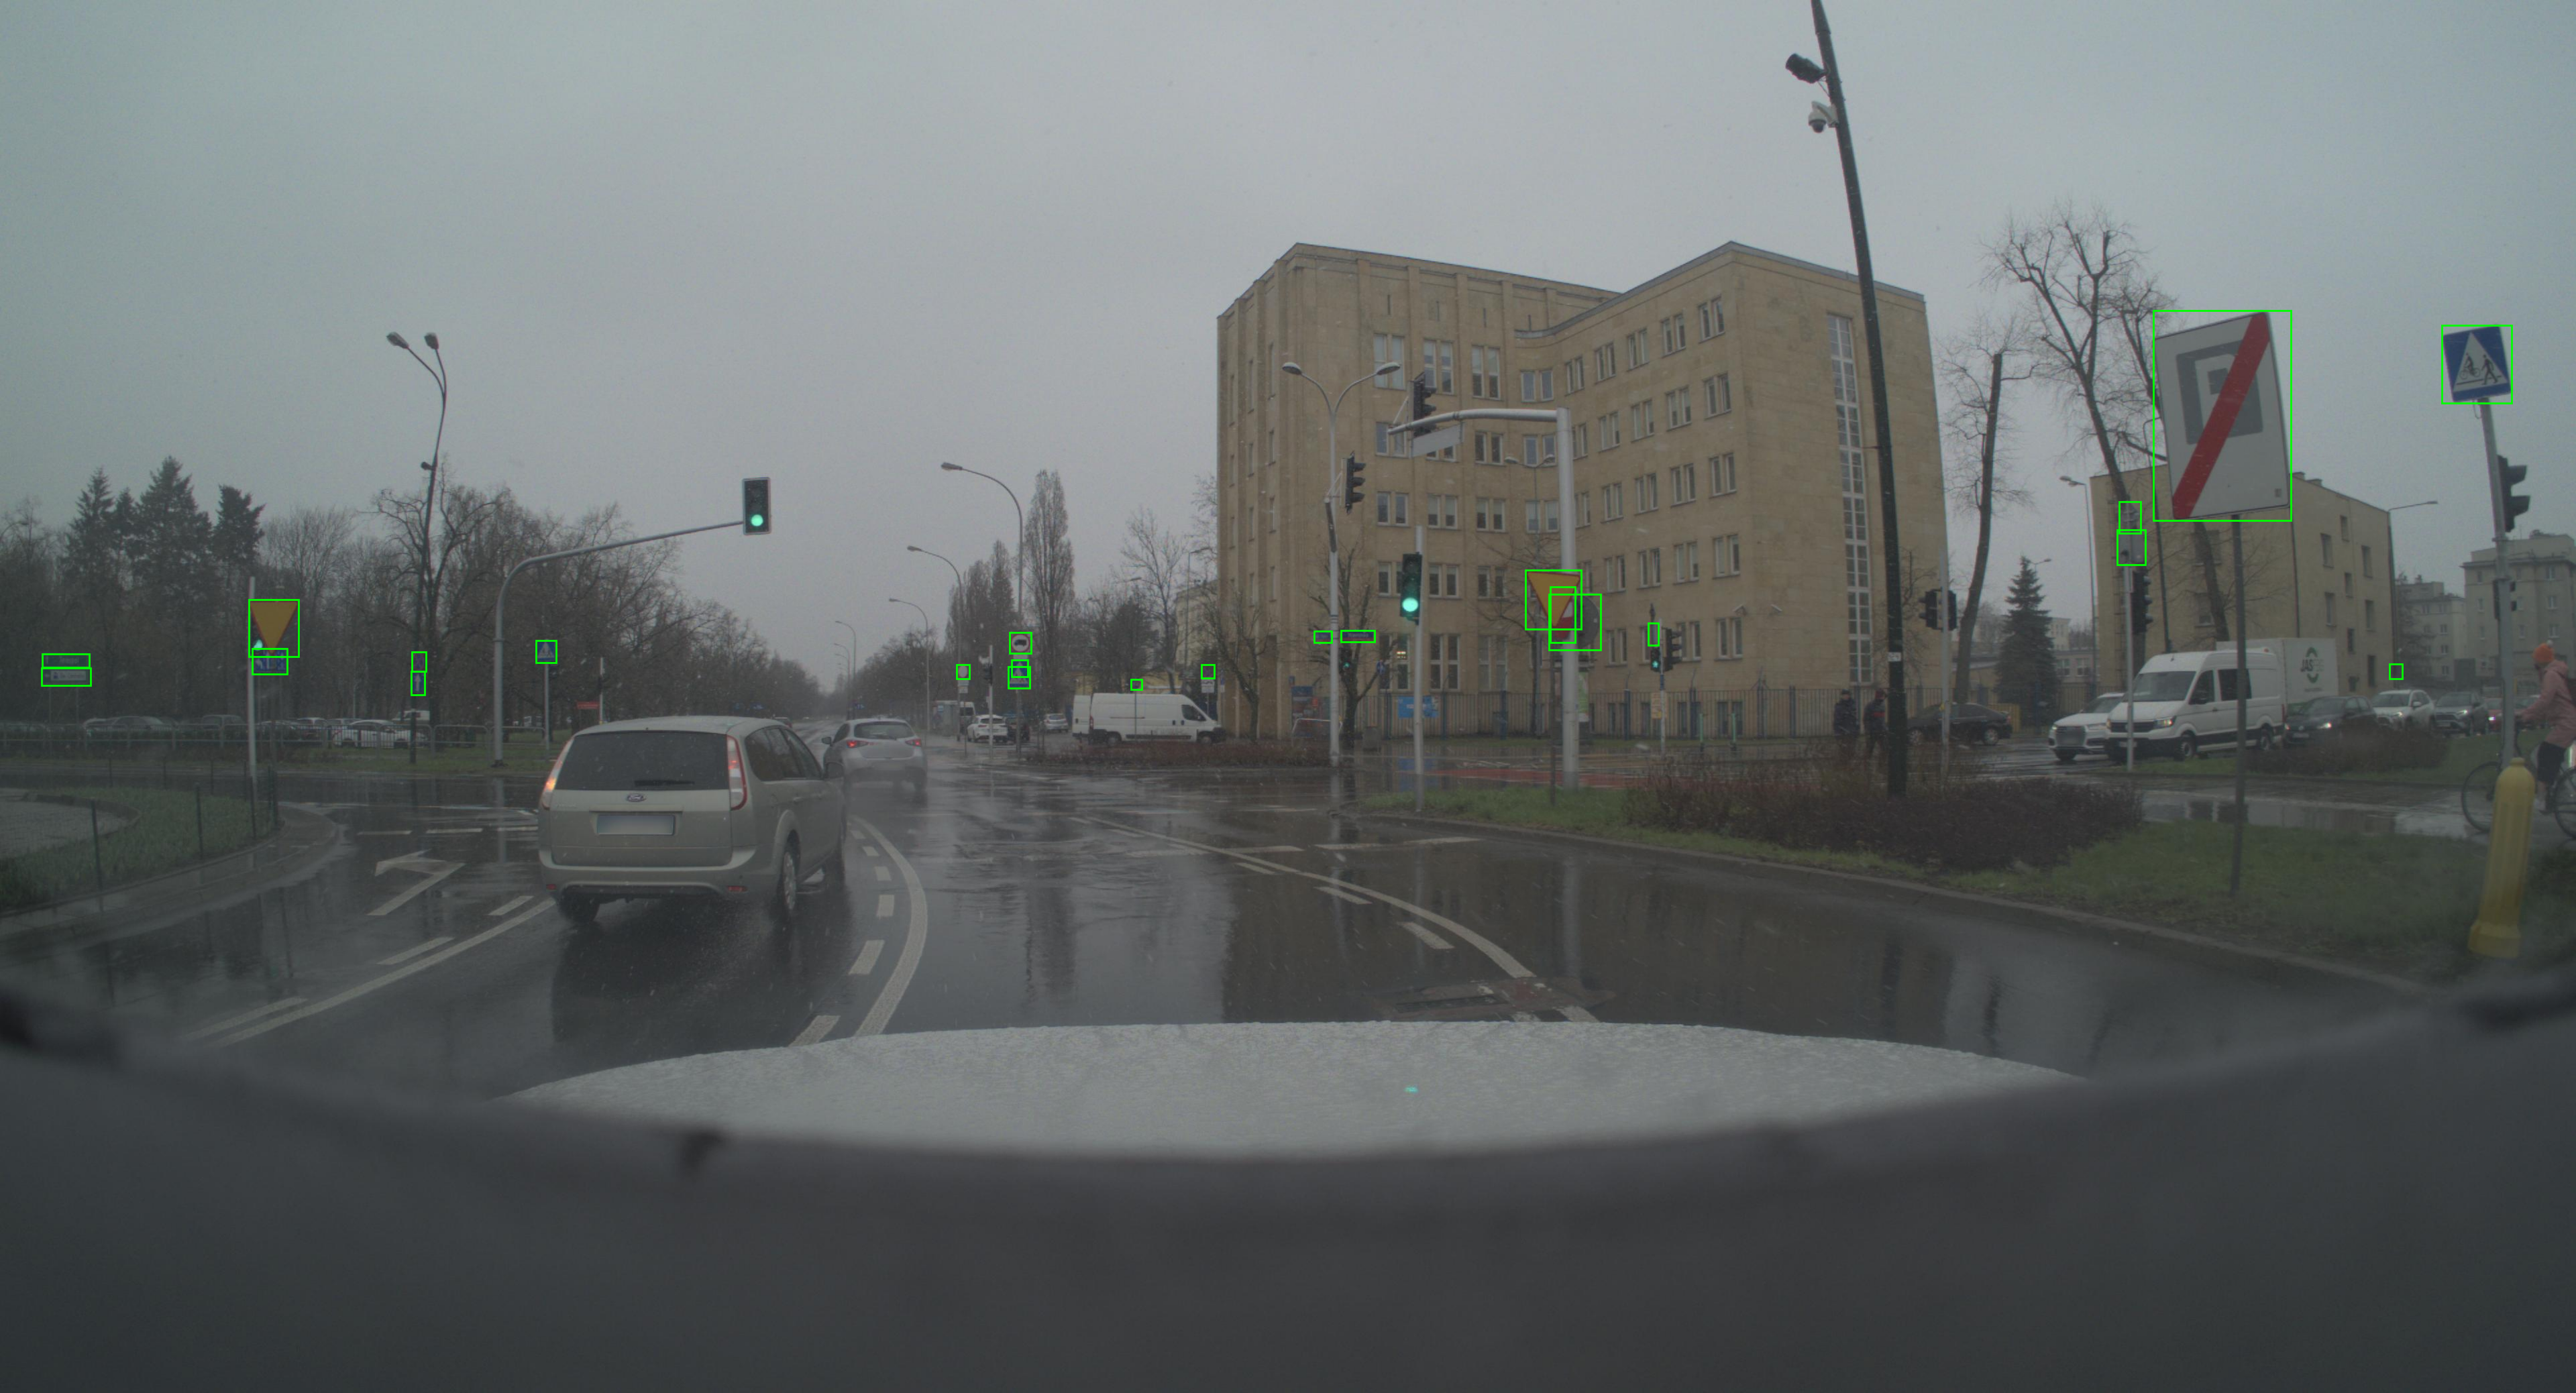
\includegraphics[width=0.49\textwidth]{images/bt4/000742.png} \\
        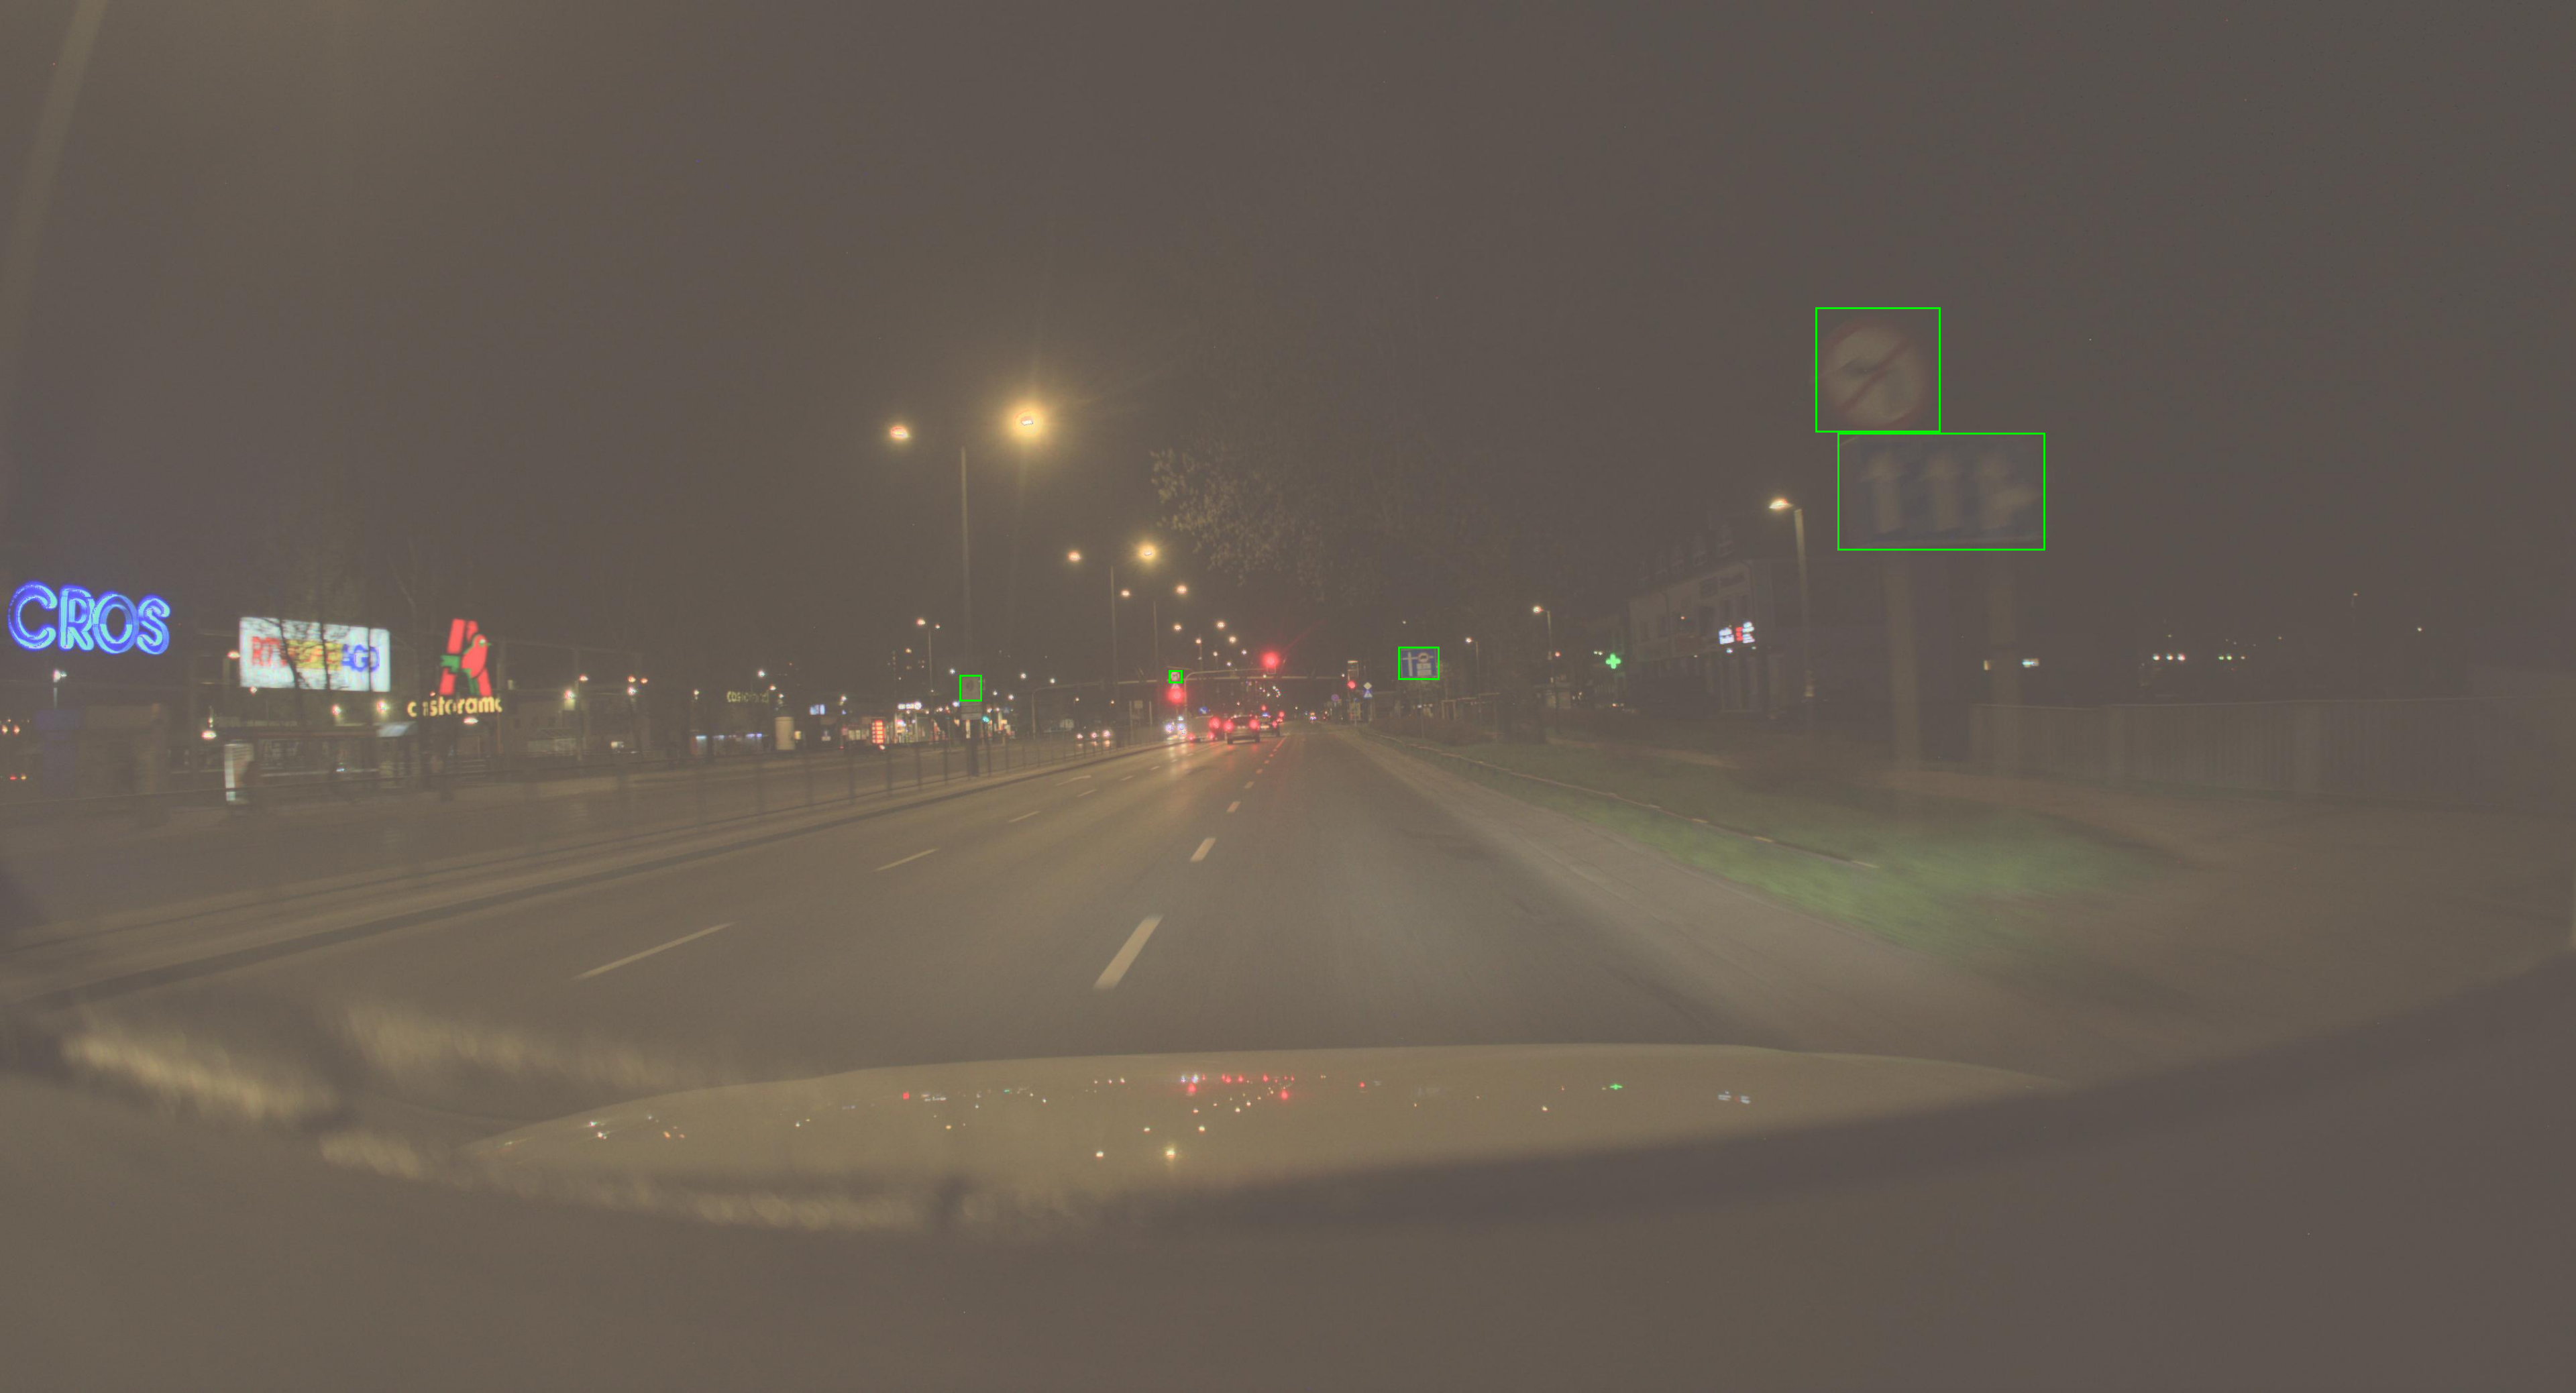
\includegraphics[width=0.49\textwidth]{images/bt4/001955.png} &
        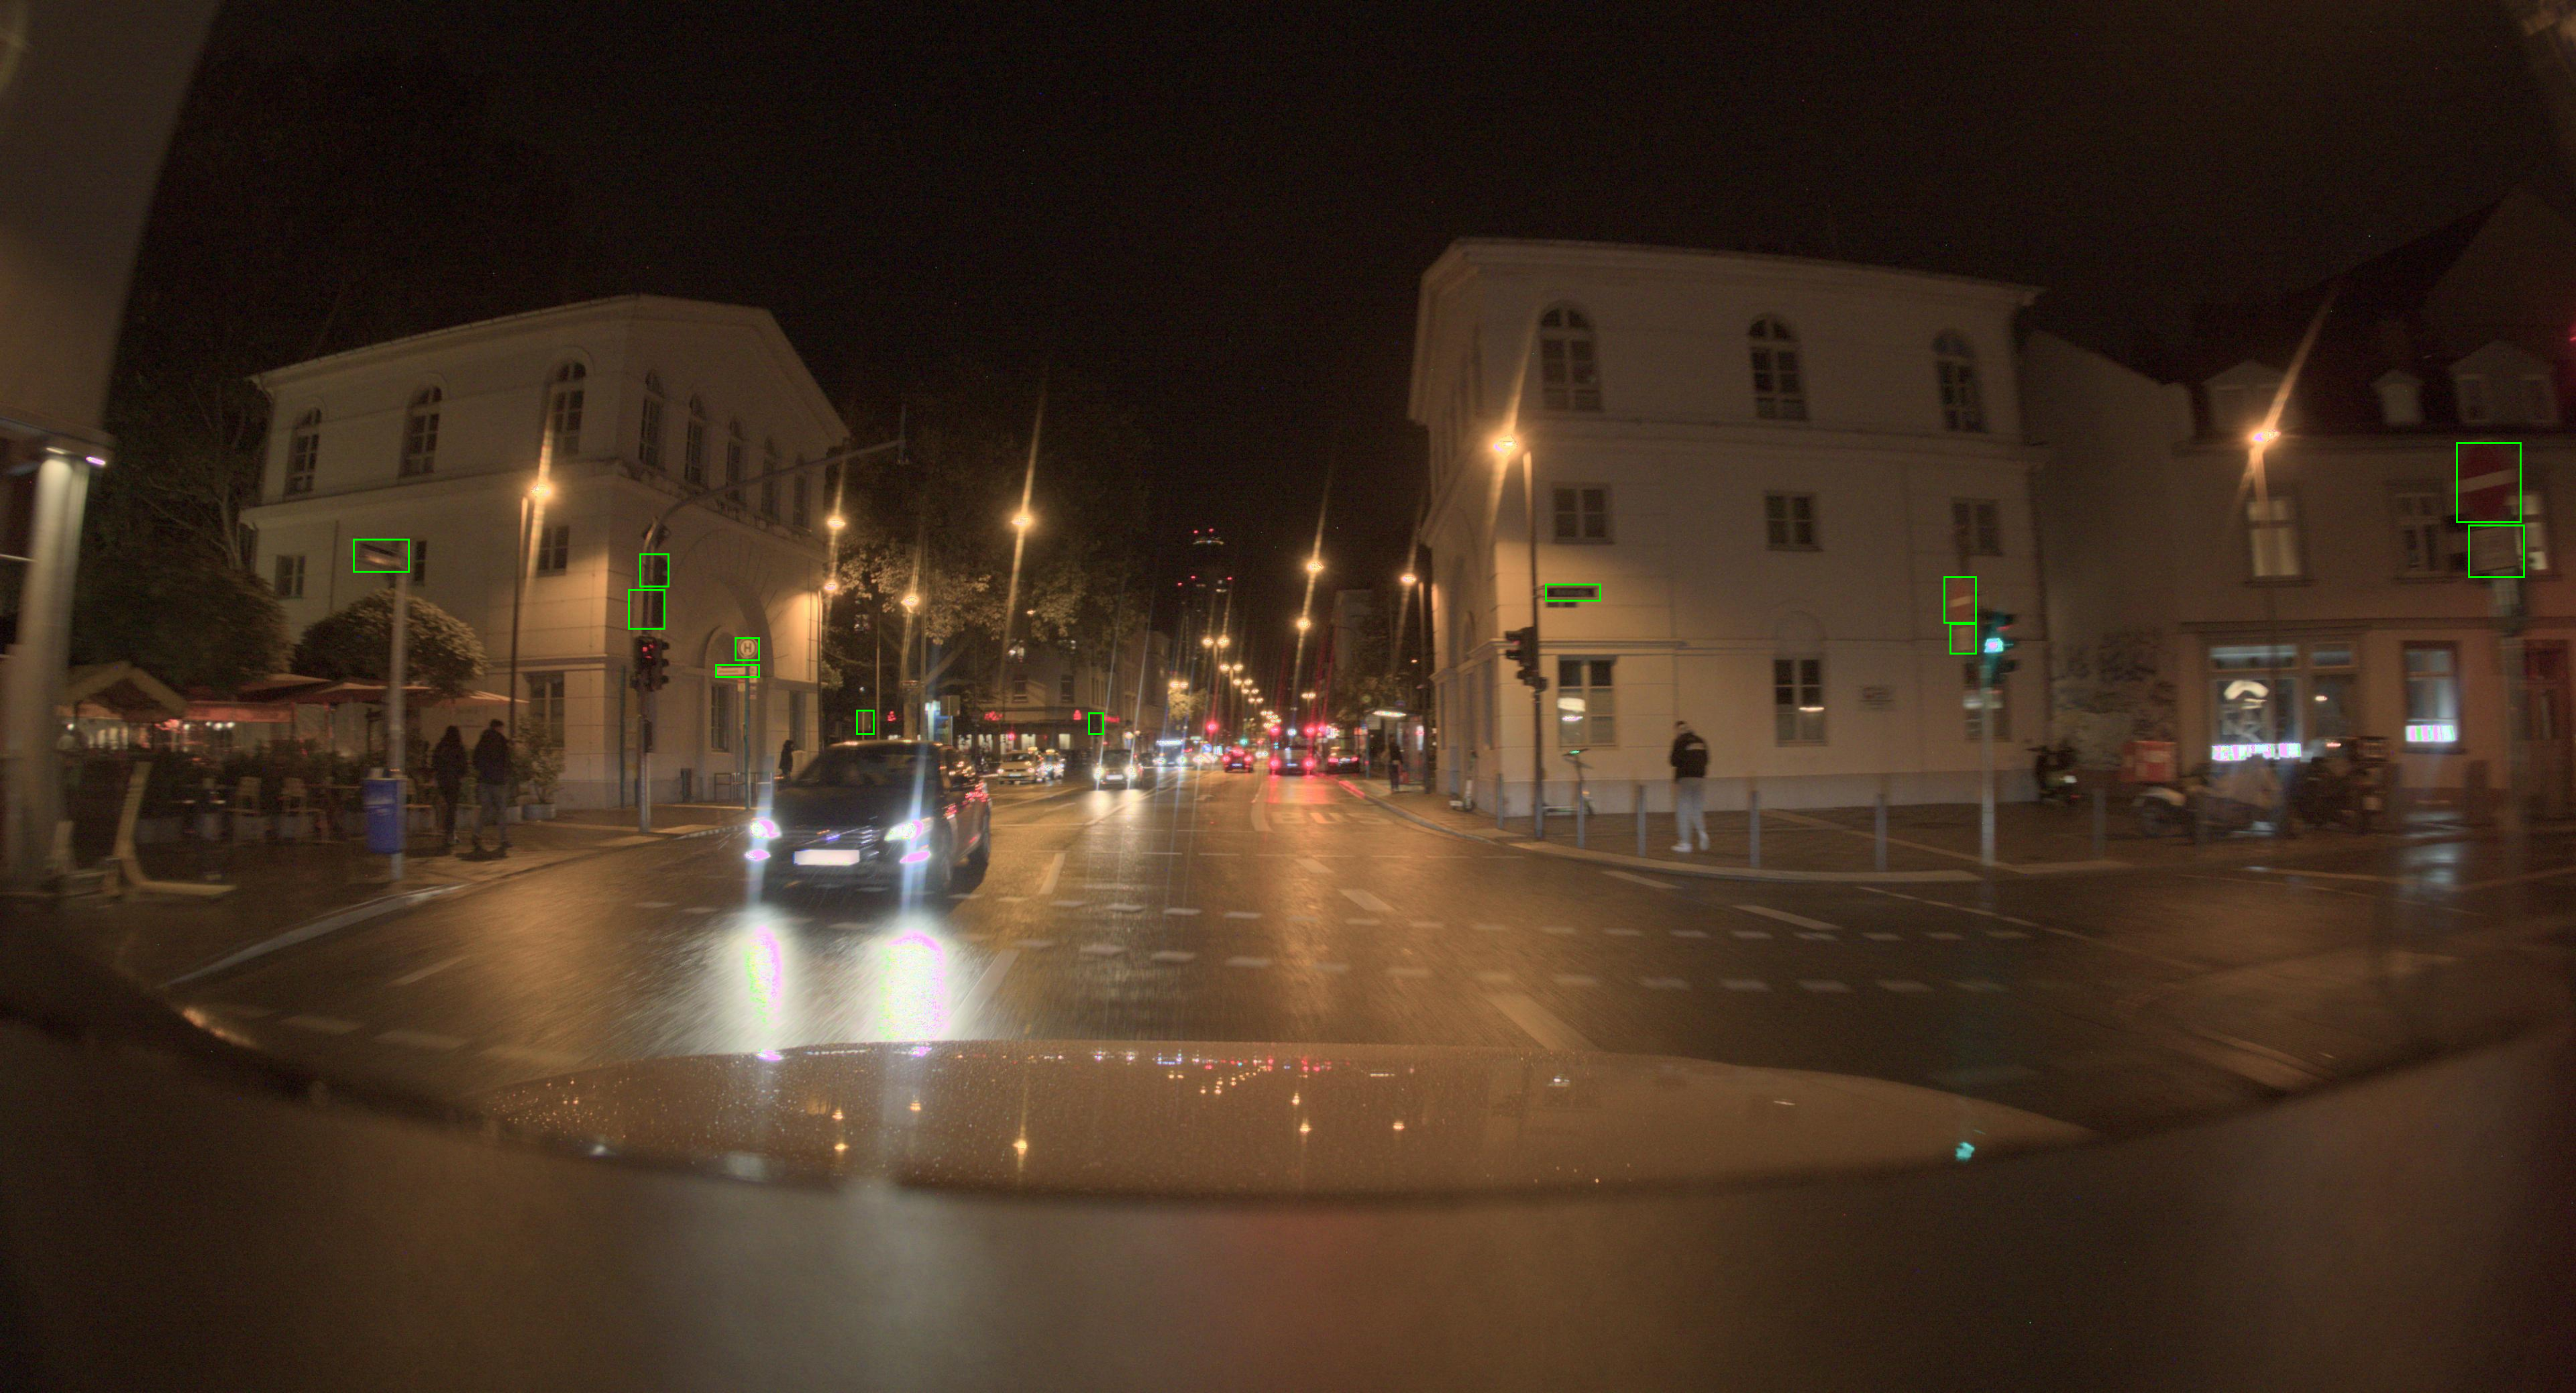
\includegraphics[width=0.49\textwidth]{images/bt4/002152.png} \\
    \end{tabular}
    \caption{Ejemplos de imágenes del dataset \texttt{bt4} con sus bounding boxes.}
    \label{fig:bt4_examples}
\end{figure}


\subsection{Diseño de los entrenamientos}
Dado que el entrenamiento de una red neuronal profunda desde cero requiere millones de imágenes y una potencia de computación masiva, hemos optado por la técnica de \textbf{Transfer Learning}.
Este proceso consiste en inicializar el modelo con pesos pre-entrenados en el dataset COCO (que contiene 80 clases generales y millones de instancias). Para adaptarlo a nuestro dominio, realizamos un \textit{Fine-Tuning}:

\begin{enumerate}
    \item Se sustituye la última capa de la cabecera (diseñada para 80 clases) por una nueva capa inicializada aleatoriamente diseñada para detectar una única clase: \texttt{TrafficSign}.
    \item Se entrenan con una tasa de aprendizaje baja las capas del Backbone para conservar la capacidad de extracción de características básicas (bordes, texturas).
    \item Se entrena la red completa con nuestro dataset curado (\texttt{bt4}) para que el modelo especialice sus pesos en la morfología específica de las señales de tráfico.
\end{enumerate}

\subsubsection{Hiperparámetros de entrenamiento}
Durante la fase experimental, se han ajustado los siguientes hiperparámetros clave que determinan el comportamiento del entrenamiento:

\begin{itemize}
    \item \textbf{Tamaño de Imagen:} Se fijó en $1024 \times 1024$ píxeles para equilibrar la resolución suficiente para detectar señales pequeñas
            y la velocidad de entrenaminento y uso de memoria.
    
    \item \textbf{Épocas (\texttt{epochs}):} Representa el número de veces que el modelo ve el dataset completo. 
     Se configuró un máximo de 200 épocas, utilizando un mecanismo de early stopping
     (paciencia = 15) para detener el entrenamiento si el modelo dejaba de mejorar, 
     evitando así el sobreajuste.
    
    \item \textbf{Batch Size:} Define cuántas imágenes procesa la GPU simultáneamente antes de actualizar 
    los pesos. Se ajustó en función de la capacidad de la memoria VRAM (16 para el modelo Nano, 8 para el Medium), buscando un equilibrio entre la estabilidad del gradiente y el uso de memoria.
    
    \item \textbf{Escala del Modelo:} en este proyecto comparamos las variantes 
    \textit{Nano} (la más ligera, $6.5\, MB$) y \textit{Medium} ($52.1\, MB$) para evaluar el impacto de la complejidad 
    del modelo en la capacidad de detección.

    \item \textbf{Confianza:} umbral de confianza mínimo para considerar una predicción como válida.
    Se mantiene por defecto en 0.25 durante el entrenamiento y validación.
\end{itemize}

\subsubsection{Métricas de evaluación}

Para evaluar el rendimiento de los modelos utilizamos
el sistema de métricas integrado en YOLOv8, basado en las métricas estándar de la comunidad
de visión por computador, especialmente las definidas en el benchmark COCO (Common Objects in Context).
Además, utilizamos la herramienta \texttt{Weights \& Biases} para registrar y visualizar las métricas. Estas
se dividen en dos tipos: funciones de pérdida (utilizadas para optimizar los pesos de la red) y
métricas de rendimiento (utilizadas para evaluar la calidad de las predicciones).

Como función de pérdida, YOLOv8 utiliza una combinación ponderada de tres componentes principales:
\begin{itemize}
    \item \textbf{Pérdida de Caja (Box Loss):} mide el error en la localización de las coordenadas de las bounding
    boxes predichas respecto a las reales utilizando la función CIoU (Complete IoU). Es una métrica
    que combina la superposición, la distancia entre centros y la proporción de aspecto.
    \item \textbf{Pérdida de Clasificación (Cls Loss)}: función de pérdida estándar de entropía cruzada
    que mide el error en la predicción de la clase del objeto. Dado que trabajamos con una única clase,
    esta pérdida tiene en solo tiene en cuenta la probabilidad asignada a la clase \texttt{TrafficSign}.
    \item \textbf{Pérdida DFL (Distribution Focal Loss):} métrica específica de YOLOv8 que refina 
    la precisión de las coordenadas de las cajas predichas modelando una distribución de probabilidad 
    de los bordes. Utilizando una distribución de probabilidad en lugar de valores puntuales,
    se coonsigue un aprendizaje menos sensible a los errores de un solo píxel comunes en la detección de
    objetos pequeños.
\end{itemize}

Por otro lado, las métricas de rendimiento utilizadas para evaluar la calidad de las predicciones son:
\begin{itemize}
    \item \textbf{Precision:} proporción de detecciones correctas entre todas las predicciones realizadas.
    \item \textbf{Recall:} proporción de señales reales que han sido correctamente detectadas.
    \item \textbf{mAP50 (Mean Average Precision at IoU=0.50):} precisión media calculada considerando una predicción 
    como si IoU $\geq$ 0.50.
    \item \textbf{mAP50-95:} precisión media calculada promediando los valores de mAP a diferentes umbrales de IoU 
    desde 0.50 hasta 0.95 en incrementos de 0.05.
\end{itemize}
La métrica final más importante es el \textbf{mAP50-95}, ya que refleja tanto la capacidad de detección como la precisión en la localización espacial de las señales.

\subsection{Reentrenamiento y resultados}

Como comentamos en apartados anteriores, hemos entrenado dos variantes del modelo YOLOv8: \textit{Nano} y \textit{Medium}. 
Se ha utilizando una GPU NVIDIA RTX 4090 con 24 GB de VRAM para el entrenamiento. 

\subsubsection{Curvas de pérdida}

La progresión de las funciones de pérdida durante el entrenamiento se muestra en la Figura \ref{fig:loss_curves}.
Se observa una disminución constante de las pérdidas DFL, de clasificación y de caja a lo largo de las épocas,
lo que indica que ambos modelos aprenden a localizar correctamente las señales. 
El modelo Medium (línea verde) reduce el error de manera más eficiente (con respecto a
la cantidad de épocas) y alcanza pérdidas finales más bajas que el modelo Nano (línea azul). Esto sugiere,
como era previsible, una mayor capacidad de aprendizaje debido a su mayor complejidad.
Las gráficas de validación confirman que no hay sobreajuste, ya que estas descienden en concordancia 
con las de entrenamiento.

\begin{figure}[H]
    \centering
    \begin{tabular}{cc}
        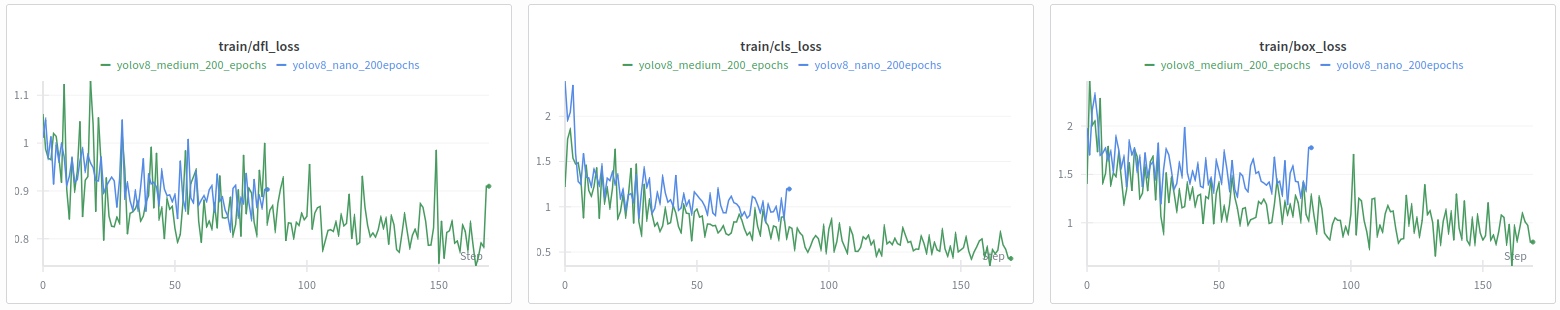
\includegraphics[width=0.9\textwidth]{images/bt4/train_loss.png} \\
        (a) Training loss \\
        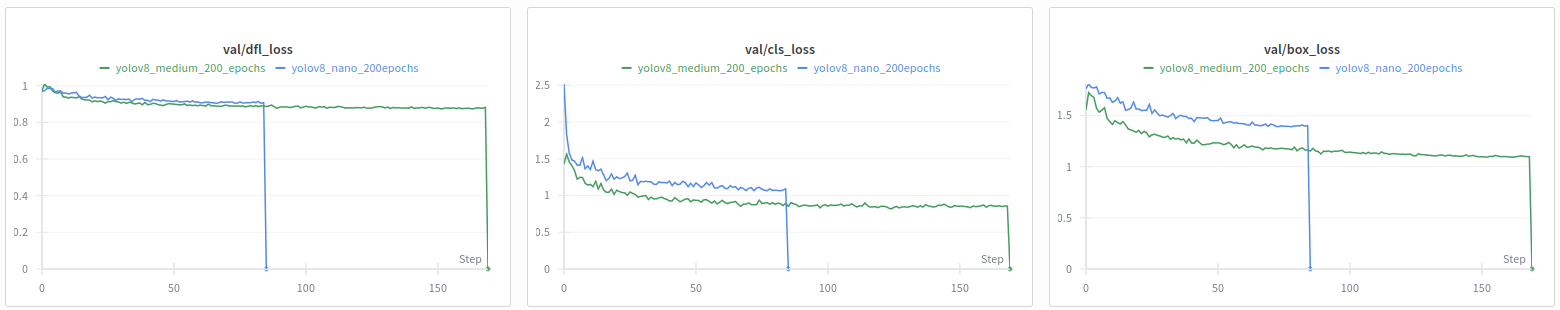
\includegraphics[width=0.9\textwidth]{images/bt4/val_loss.png} \\
        (b) Validation loss 
    \end{tabular}
    \caption{Curvas de pérdida durante el entrenamiento para las variantes (a) YOLOv8 Nano y (b) YOLOv8 Medium.}
    \label{fig:loss_curves}
\end{figure}

\subsubsection{Métricas de rendimiento}

En la siguiente tabla \ref{tab:training_summary} se resumen los parámetros clave y los resultados obtenidos
durante los entrenamientos de ambas variantes del modelo YOLOv8.

\begin{table}[H]
    \centering
    \begin{tabular}{lcc}
        \toprule
        \textbf{Parámetro} & \textbf{YOLOv8 Nano} & \textbf{YOLOv8 Medium} \\
        \midrule
        Tamaño del modelo & 6.5 MB & 52.1 MB \\
        Batch Size & 16 & 8 \\
        Épocas (con early stopping) & 85 & 169 \\
        Tiempo total de entrenamiento & 13 minutos & 1 hora 15 minutos \\
        Mejor Precision alcanzada & 64.31\% & 72.10\% \\
        Mejor Recall alcanzado & 38.91\% & 50.92\% \\
        Mejor mAP50 alcanzado & 43.74\% & 57.47\% \\
        Mejor mAP50-95 alcanzado & 24.91\% & 36.52\% \\
        \bottomrule
    \end{tabular}
    \caption{Resumen de los entrenamientos realizados con YOLOv8 Nano y Medium.}
    \label{tab:training_summary}
\end{table}

Como observamos, el modelo Medium supera significativamente al Nano en todas las métricas clave. 
En cuanto a la métrica mAP50-95, la mejora es de casi 12 puntos porcentuales (46.61\% relativa al base) con
un coste del 676.92\% de tiempo de entrenamiento. A pesar de esta gran diferencia, un entrenamiento de 
una hora y cuarto sigue siendo razonable para aplicaciones prácticas, teniendo en cuenta además que estos 
modelos de base han sido preentrenados durante semanas en datasets masivos. 

La diferencia entre la precisión y el recall es notable en ambos modelos, indicando que el modelo 
es altamente preciso (cuando realiza una predicción, es muy probable que sea correcta), pero 
tiende a omitir detecciones. Podemos afirmar que el modelo es conservador en sus predicciones,
priorizando la precisión sobre la exhaustividad.

Las matrices de confusión permiten diagnosticar el tipo de error predominante. Dado que se 
trata de un problema de una sola clase, las matrices que se muestran son de $2 \times 2$, donde la primera fila/columna
corresponde a la clase \texttt{TrafficSign} y la segunda a la clase \texttt{Background} (ausencia de señal). 

\begin{figure}[H]
    \centering
    \begin{tabular}{cc}
        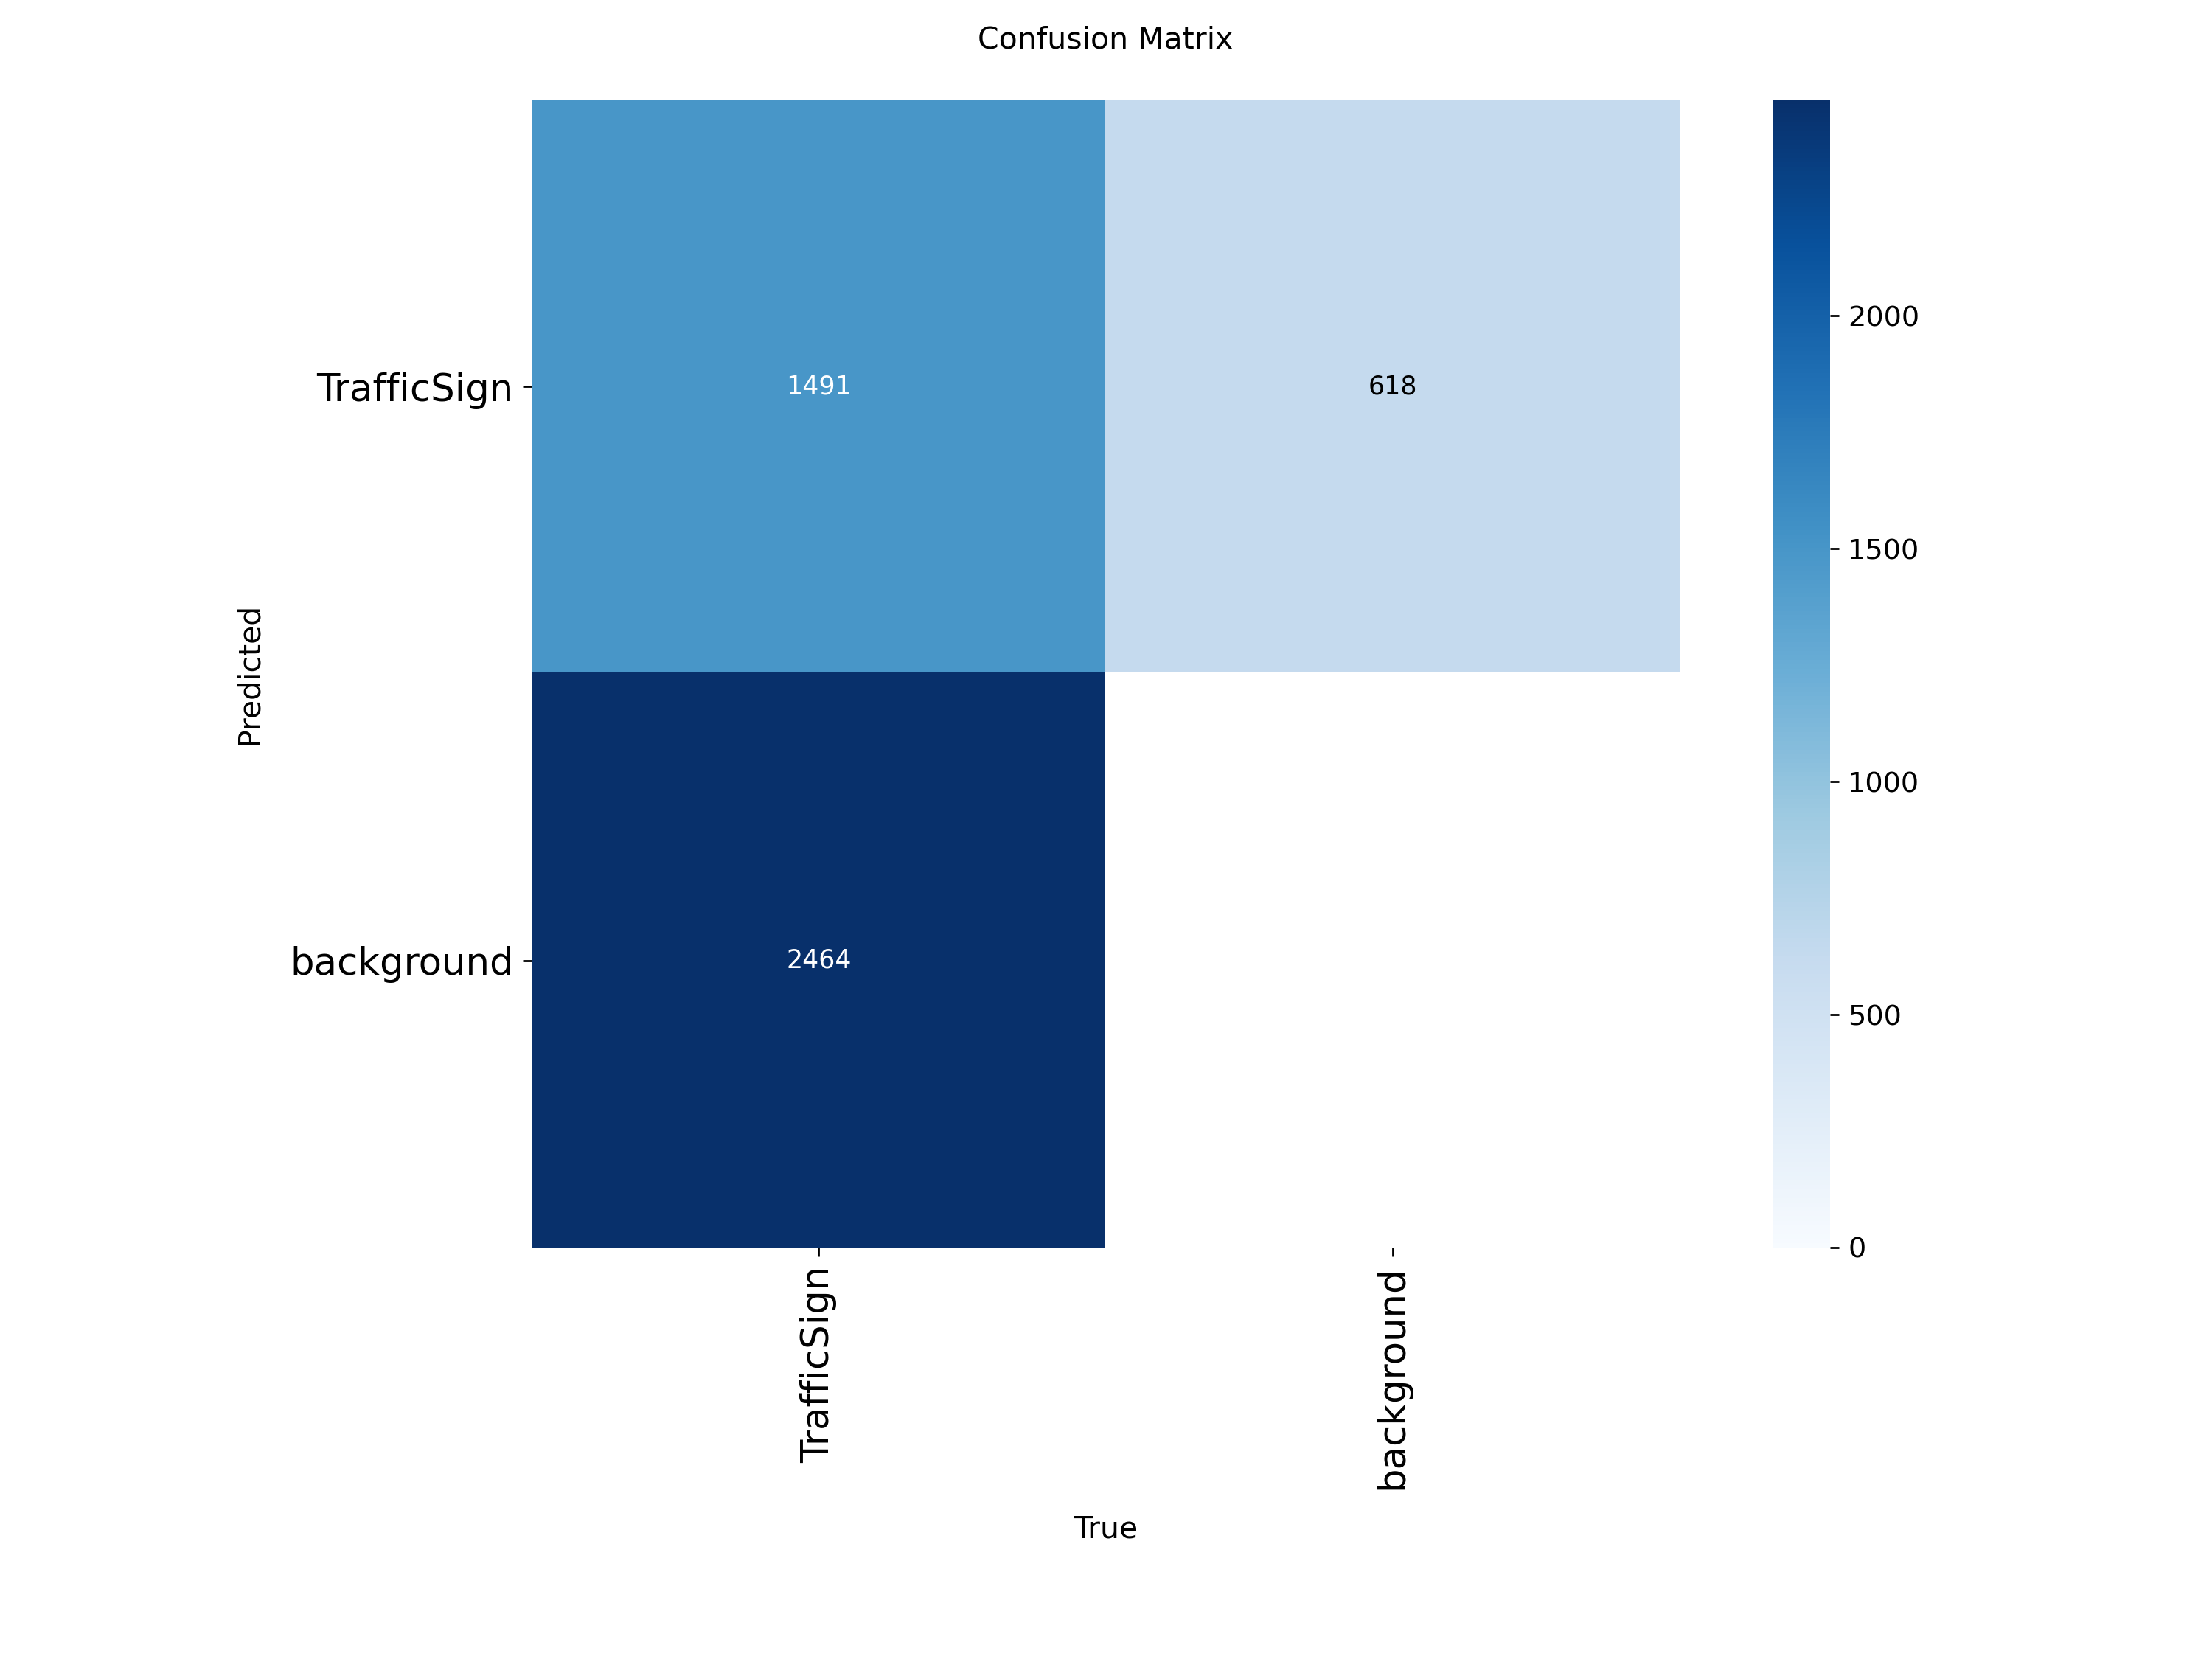
\includegraphics[width=0.5\textwidth]{images/bt4/confusion_matrix_nano.png} &
        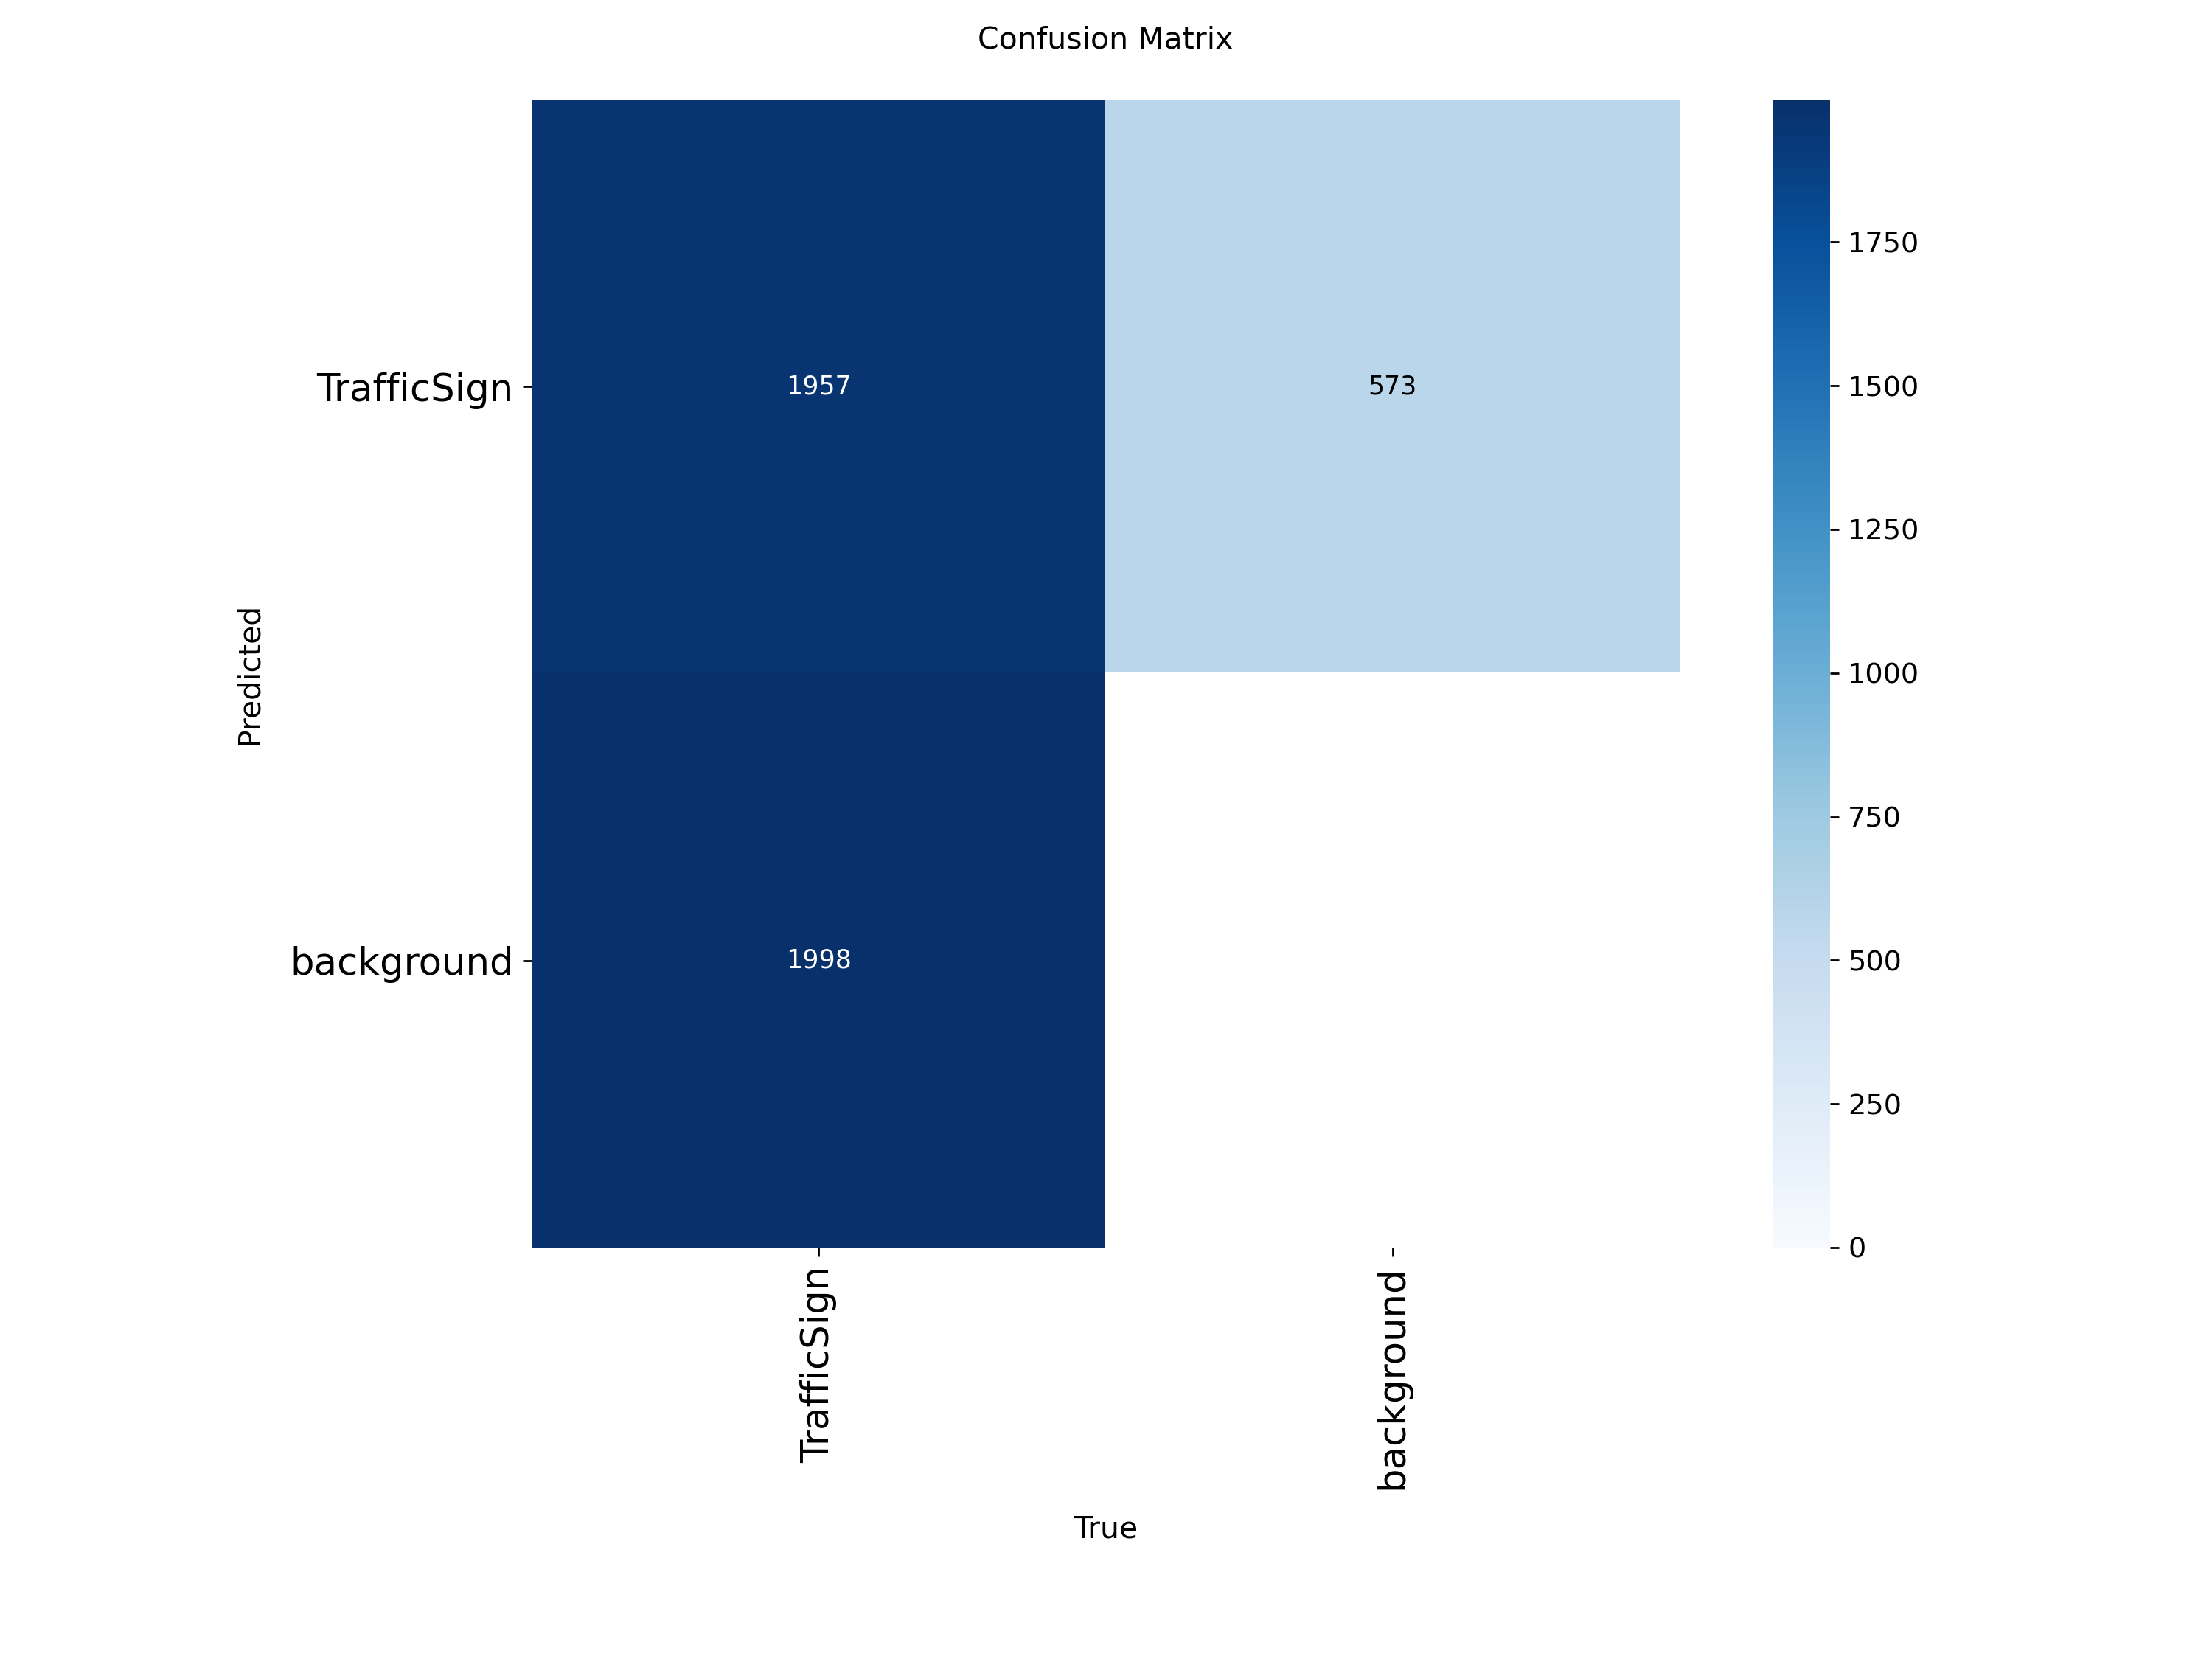
\includegraphics[width=0.5\textwidth]{images/bt4/confusion_matrix_medium.png} \\
        (a) YOLOv8 Nano & (b) YOLOv8 Medium \\
    \end{tabular}
    \caption{Matrices de confusión normalizadas para las variantes (a) YOLOv8 Nano y (b) YOLOv8 Medium.}
    \label{fig:confusion_matrices}
\end{figure}

Ambos modelos tienden a cometer más errores de falsos negativos (señales no detectadas) que falsos positivos (detecciones erróneas).
Destaca la ausencia de verdaderos negativos en ambos modelos, lo que es consistente con el hecho de que el modelo
no emite predicciones explícitas para la clase \texttt{Background}. El modelo Medium reduce significativamente los falsos negativos
en comparación con el Nano, lo que se traduce en el mayor recall observado en la tabla \ref{tab:training_summary}.

Visto de forma aislada, podría parecer que los resultados obtenidos son modestos, con un mAP50-95 del 36.52\% para el mejor modelo.
Sin embargo, es importante considerar el contexto: la detección de señales de tráfico en in imágenes de alta resolución
con la presencia de instancias muy pequeñas (señales a larga distancia) y en condiciones ambientales variadas (iluminación, oclusiones, ángulos de visión).

\subsubsection{Comparación con los modelos base}

Para evaluar el impacto del reentrenamiento, hemos comparado los modelos reentrenados con sus versiones base preentrenadas en COCO.
La evolución de las métricas clave se muestra en la imagen \ref{img:metrics}.

\begin{figure}[H]
    \centering
    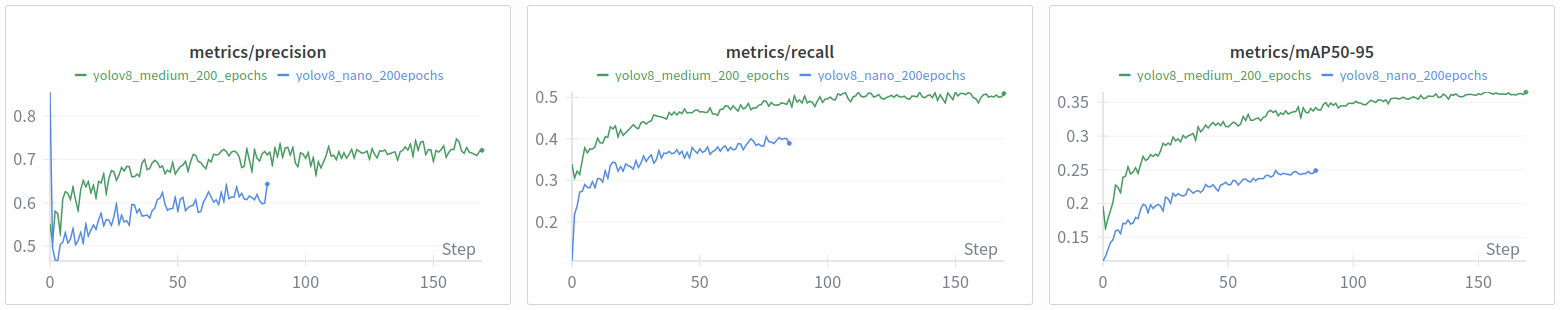
\includegraphics[width=0.99\textwidth]{images/bt4/metrics.png}
    \caption{Evolución de las métricas clave durante el entrenamiento para las variantes (a) YOLOv8 Nano y (b) YOLOv8 Medium.}
    \label{img:metrics}
\end{figure}

Al observar las gráficas, se aprecia una fase inicial de mejora rápida en el primer tercio del entrenamiento, seguida de una estabilización progresiva.
Esta rapidez inicial es en gran parte atribuible al hecho de que los modelos ya poseen una base sólida de conocimiento
(pesos y filtros convolucionales) gracias al preentrenamiento en COCO. El proceso de \textit{Fine-Tuning} permite al modelo adaptar y especializar este conocimiento
a las características específicas de las señales de tráfico presentes en nuestro dataset. Podemos comparar las métricas iniciales y finales en la siguiente tabla:

\begin{table}[H]
    \centering
    \begin{tabular}{lcccc}
        \toprule
         & \textbf{Y. Nano (Base)} & \textbf{Y. Nano (FT)} & \textbf{Y. Med. (Base)} & \textbf{Y. Med. (FT)} \\
        \midrule
        Precision & 85.55\% & 64.31\% & 54.97\% & 72.10\% \\
        Recall & 10.59\% & 38.91\% & 33.81\% & 50.92\% \\
        mAP50-95 & 11.49\% & 24.91\% & 19.58\% & 36.52\% \\
        \bottomrule
    \end{tabular}
    \caption{Comparación de métricas entre los modelos base y los reentrenados.}
    \label{tab:base_vs_finetuned}
\end{table}

La precisión inicial artificialmente alta (85.55\%) del modelo base no indica un buen rendimiento, 
sino un comportamiento extremadamente conservador: detecta muy pocas instancias (Recall ~10\%) 
pero con alta seguridad. El reentrenamiento equilibra el modelo, sacrificando esa 'falsa' 
precisión inicial para triplicar la capacidad de recuperación de objetos (Recall ~39\%).
De hecho, podemos ver en la primera gráfica de la Figura \ref{img:metrics} cómo la precisión disminuye 
bruscamente en la primera época.

\subsubsection{Rendimiento en tiempo real}

La viabilidad práctica de los modelos se confirma con el análisis de los tiempos de inferencia medidos en la GPU NVIDIA RTX 4090.
El modelo YOLOv8 Nano alcanza un tiempo promedio de inferencia de aproximadamente 5 ms por imagen, mientras que el modelo Medium
tarda alrededor de 7 ms. Dado que el umbral para aplicaciones en tiempo real suele situarse en torno a los 33 ms (30 fps), 
ambos modelos son capaces de operar en tiempo real, incluso el más complejo. La diferencia de 2 ms 
a favor del modelo Nano no justifica la pérdida de 12 puntos porcentuales en mAP50-95, por lo que
valida la elección del modelo Medium para aplicaciones prácticas. Claro está, que estos tiempos pueden variar
según la GPU utilizada y la optimización del entorno de ejecución.

\subsubsection{Comparación cualitativa}

A continuación, se muestran imágenes de ejemplo con las predicciones realizadas por ambos modelos. Mostramos
únicamente las cajas con una confianza superior al 25\% para facilitar la visualización.

\begin{figure}[H]
    \centering
    \begin{tabular}{cc}
        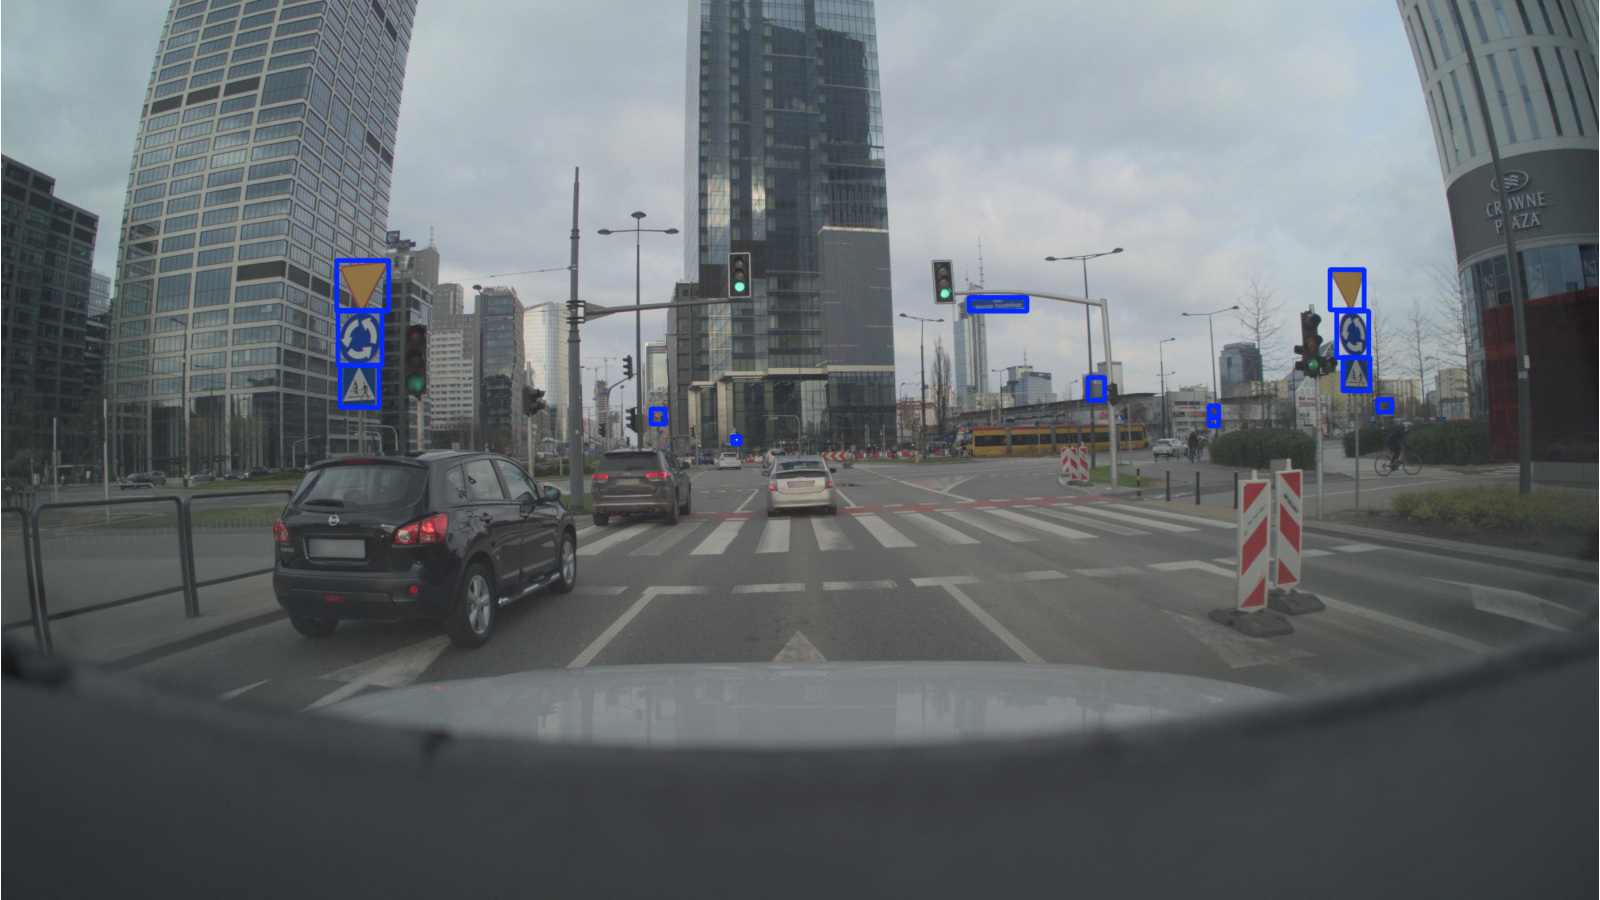
\includegraphics[width=0.45\textwidth]{images/bt4/inferencia_nano_000224.png} &
        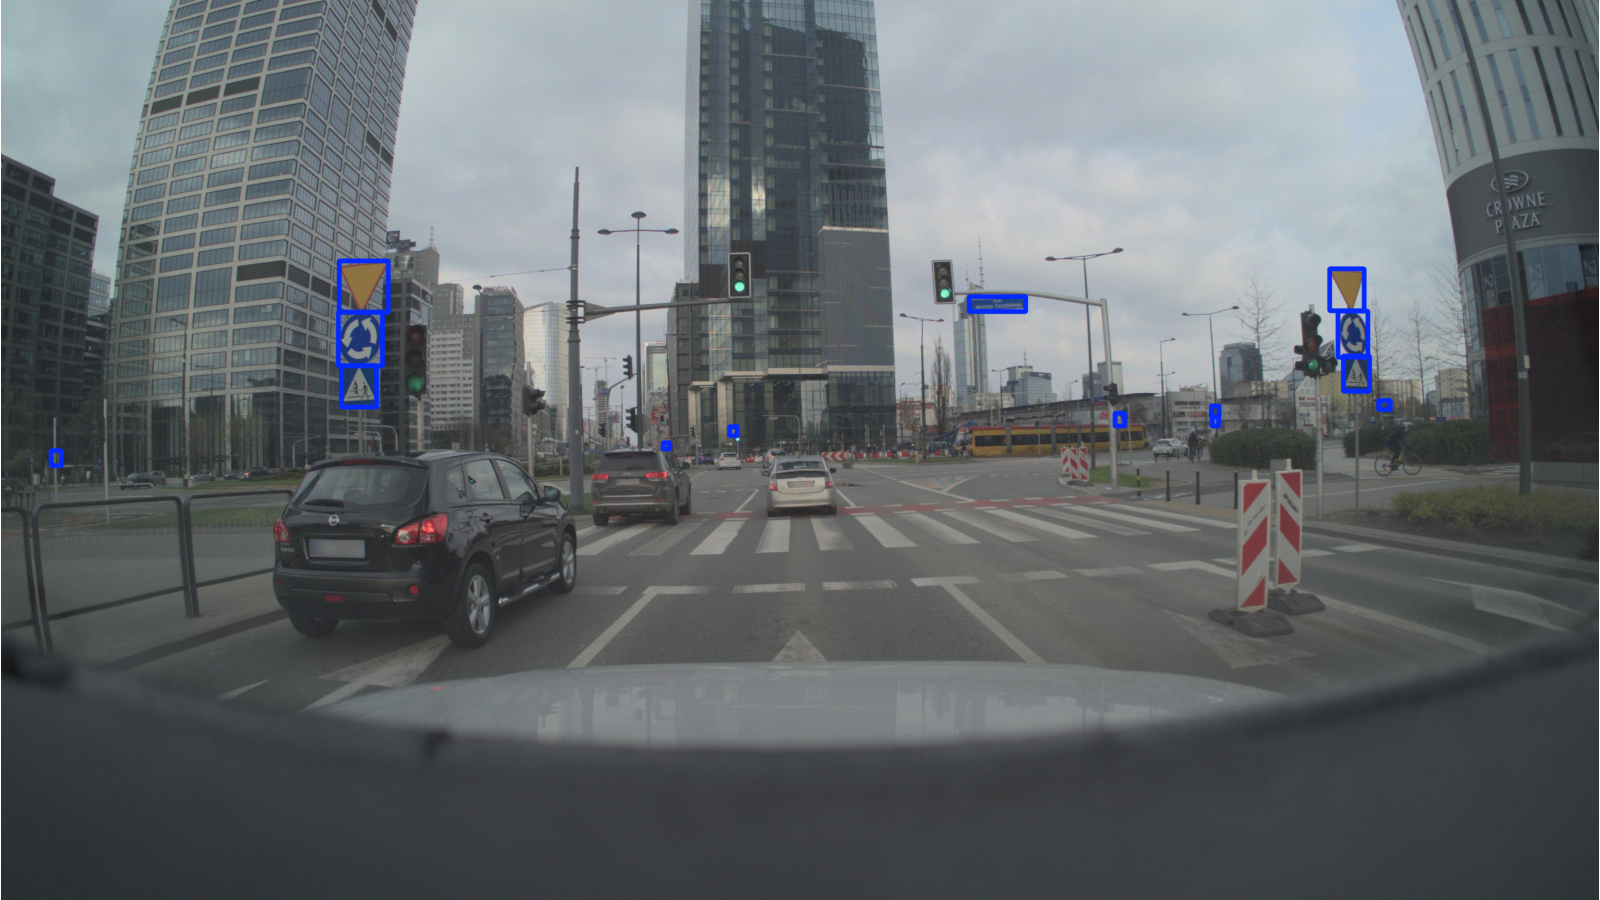
\includegraphics[width=0.45\textwidth]{images/bt4/inferencia_medium_000224.png} \\
        (a) ZOD 000224 YOLOv8 Nano & (b) ZOD 000224 YOLOv8 Medium \\
        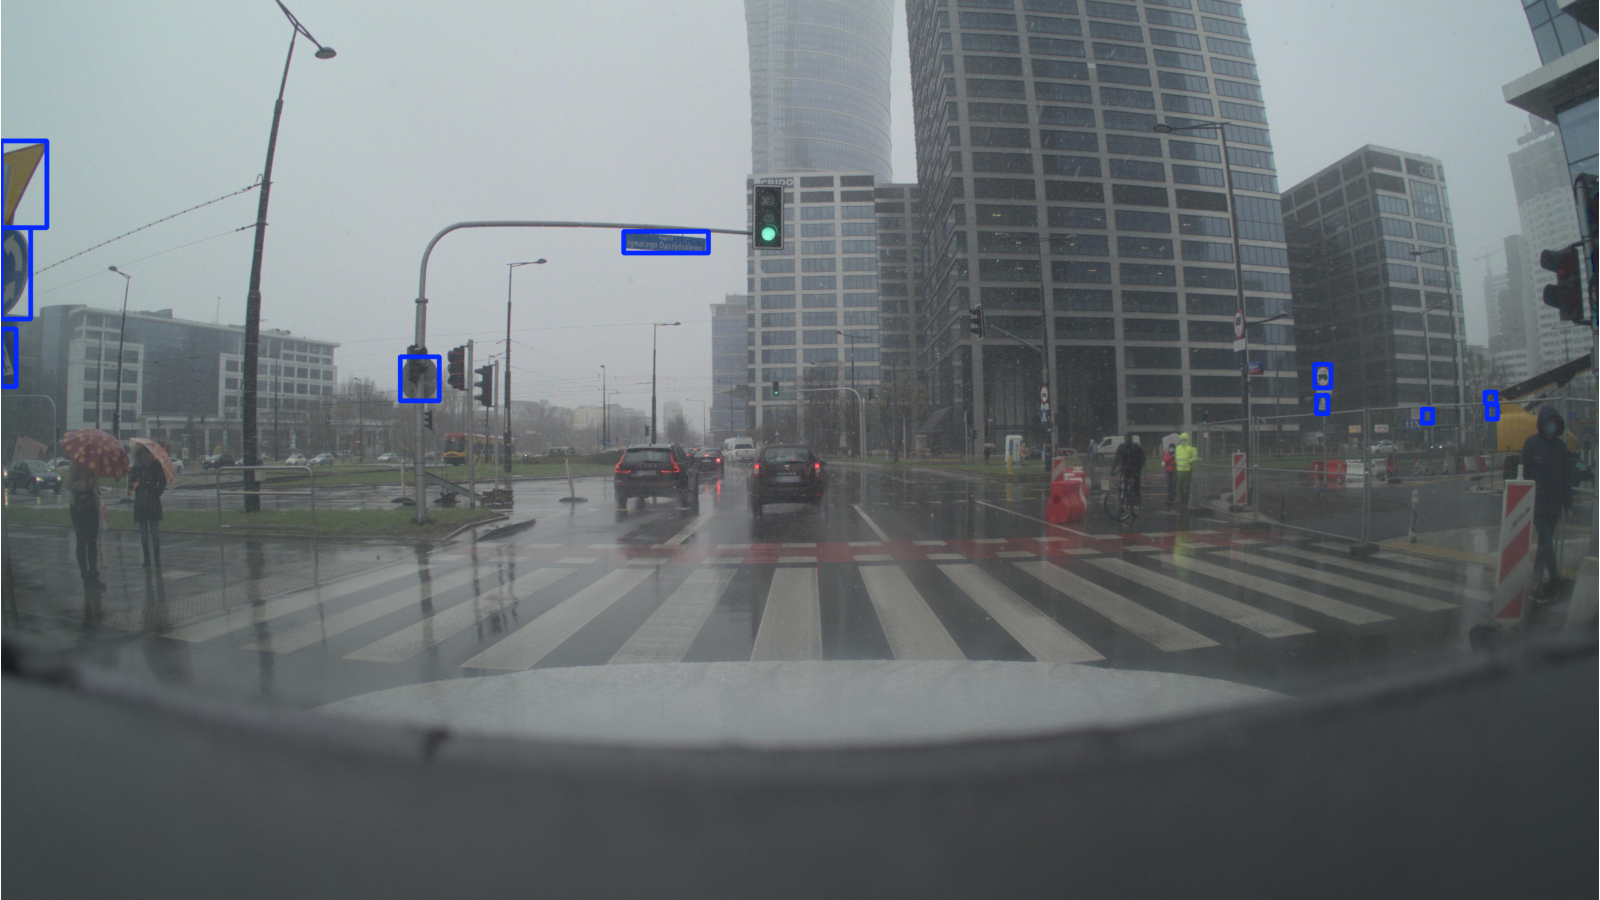
\includegraphics[width=0.45\textwidth]{images/bt4/inferencia_nano_001237.png} &
        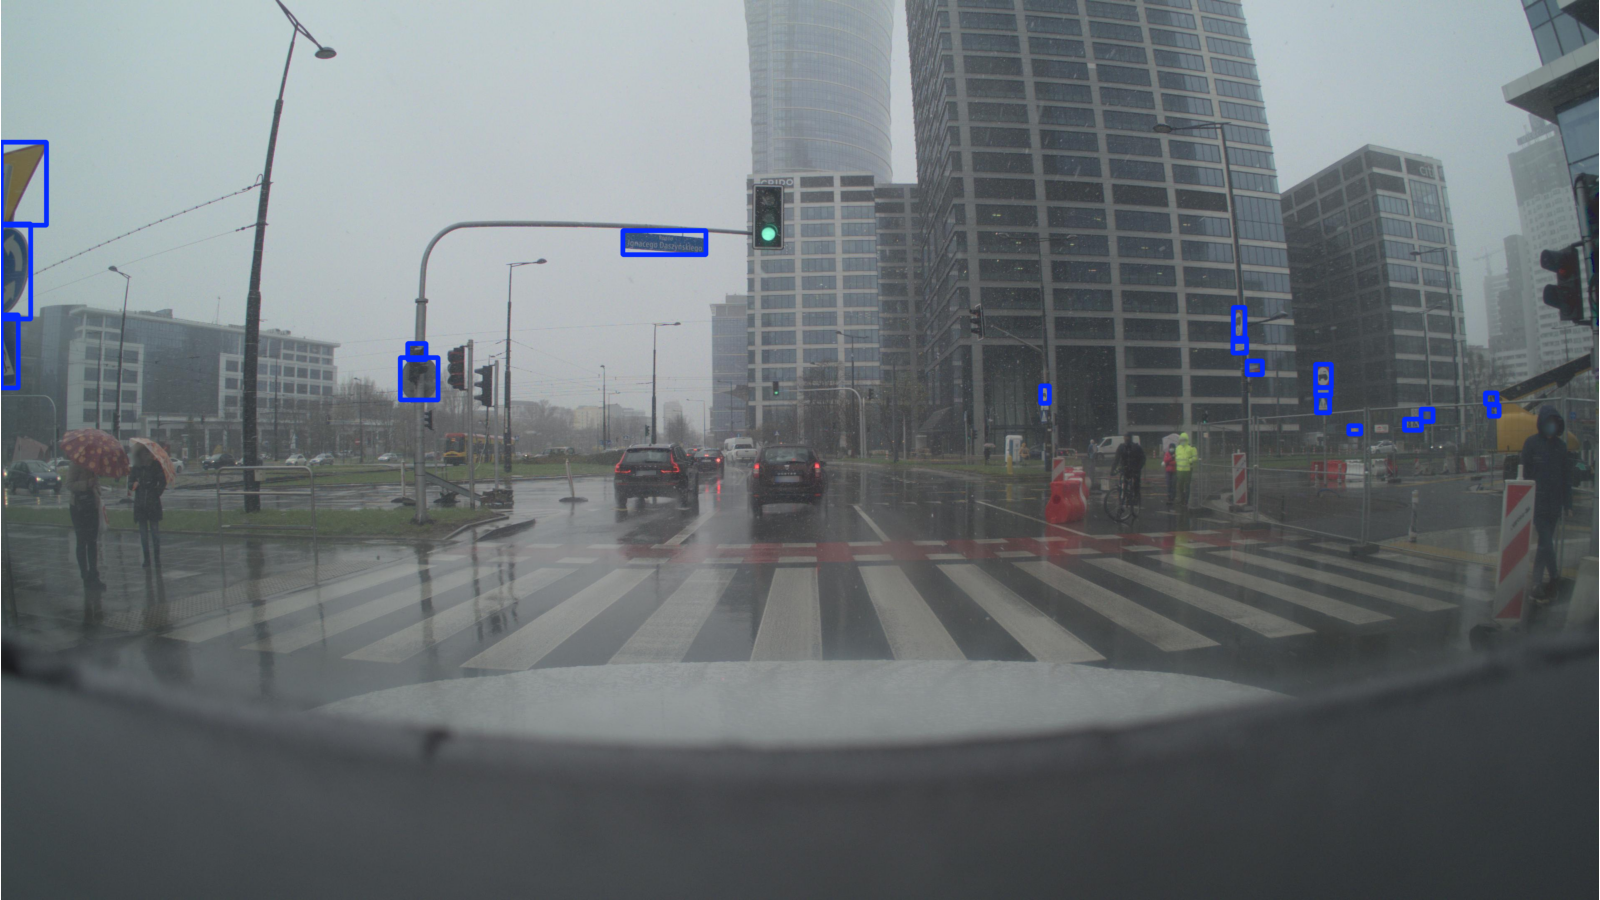
\includegraphics[width=0.45\textwidth]{images/bt4/inferencia_medium_001237.png} \\
        (c) ZOD 001237 YOLOv8 Nano & (d) ZOD 001237 YOLOv8 Medium \\
        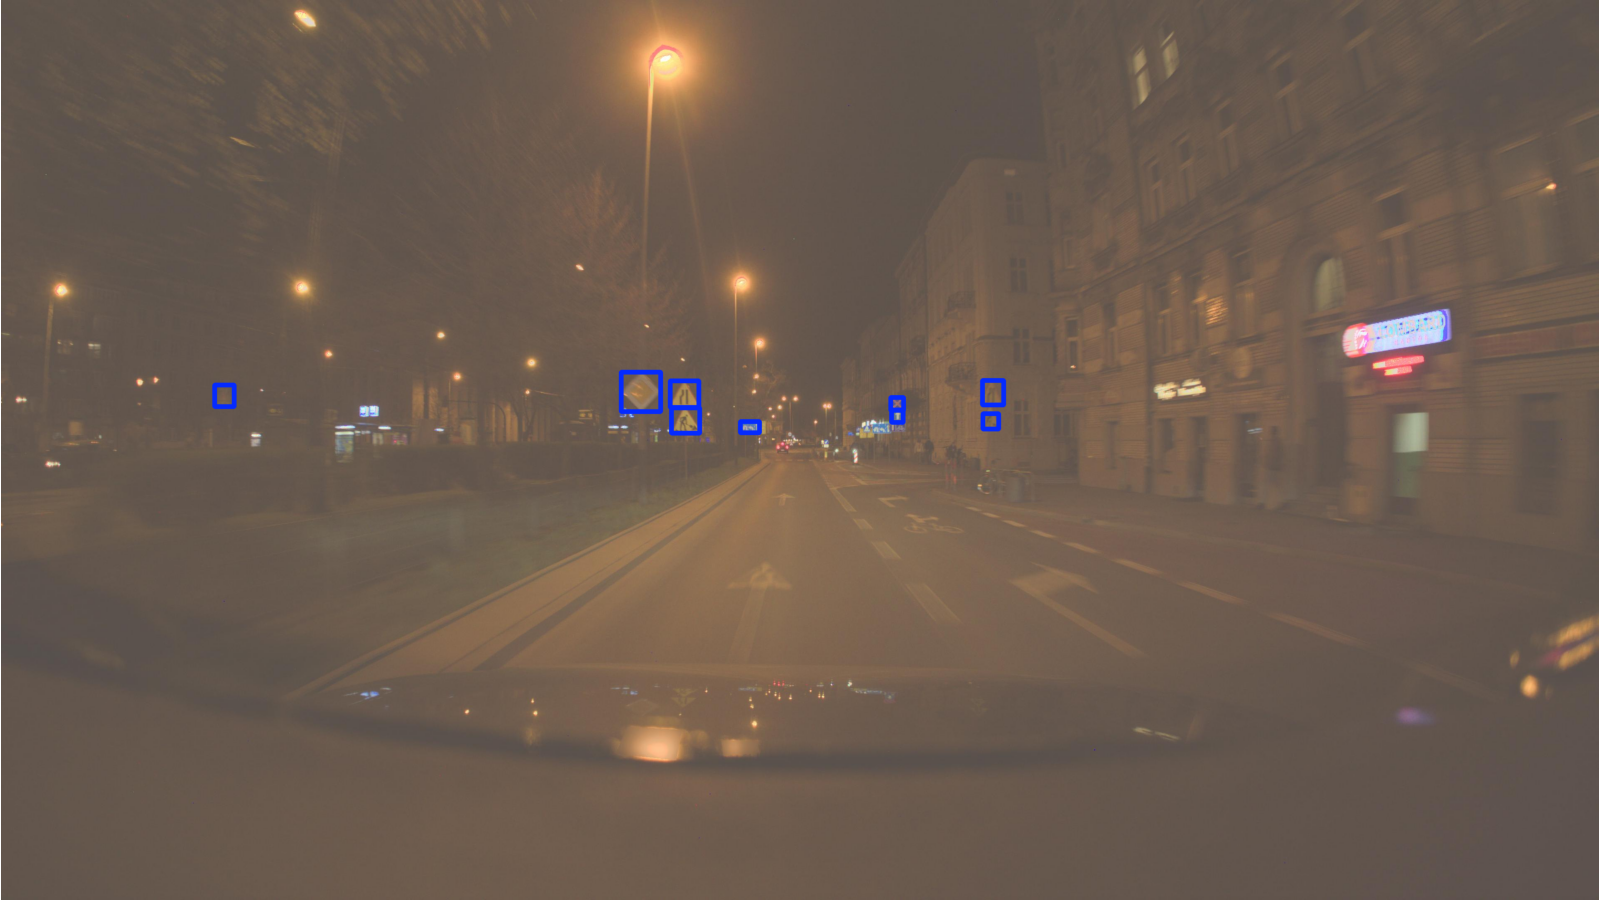
\includegraphics[width=0.45\textwidth]{images/bt4/inferencia_nano_006283.png} &
        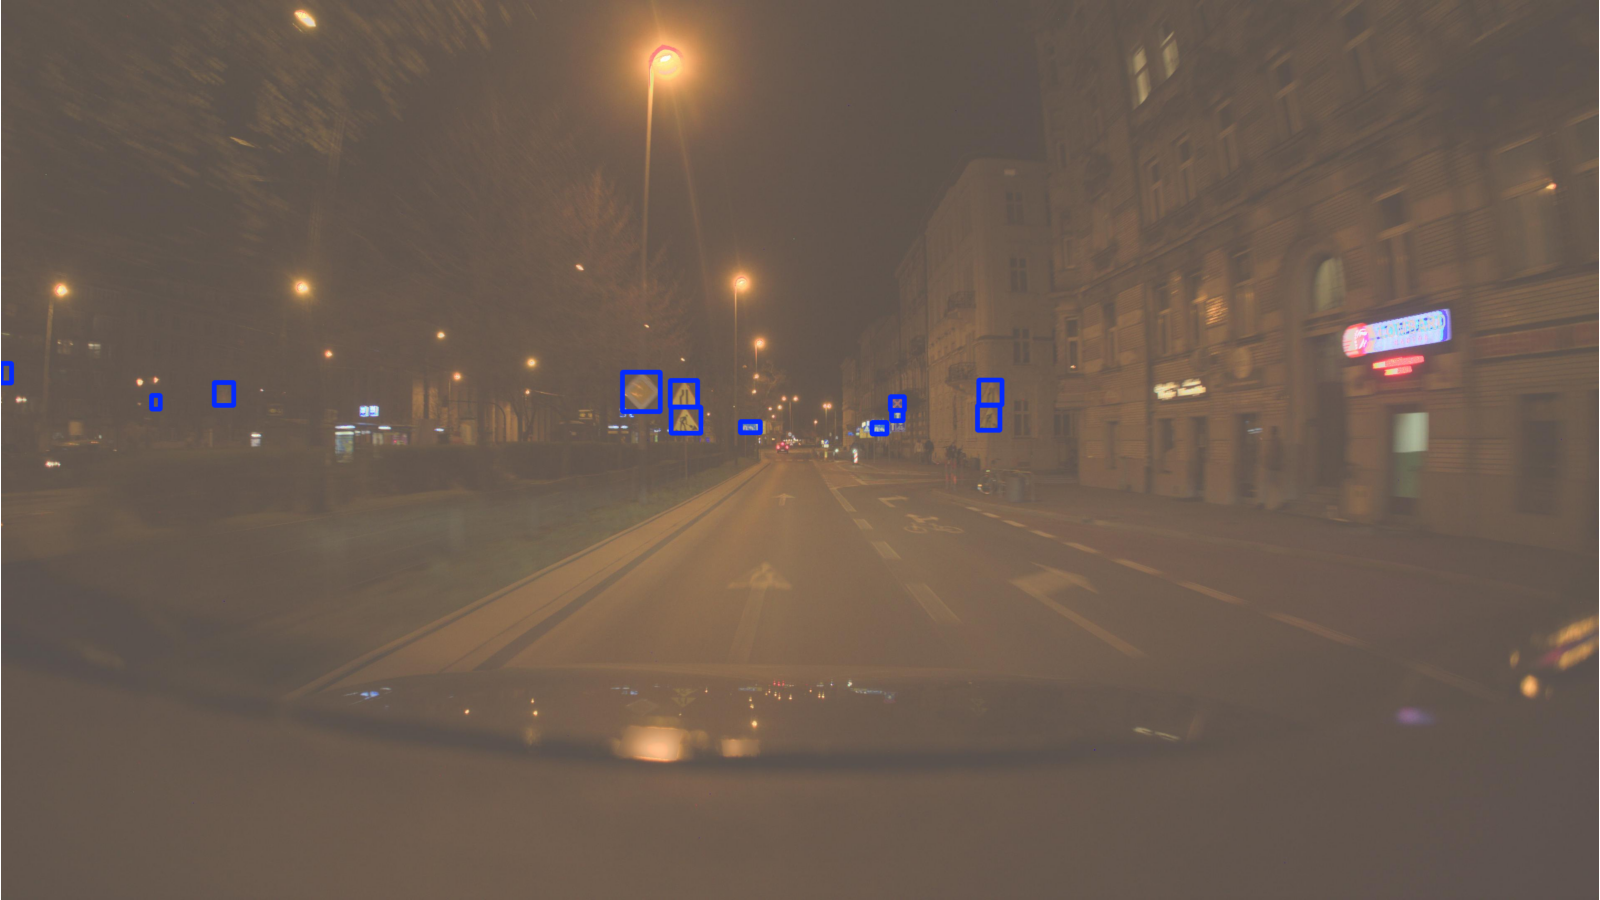
\includegraphics[width=0.45\textwidth]{images/bt4/inferencia_medium_006283.png} \\
        (e) ZOD 006283 YOLOv8 Nano & (f) ZOD 006283 YOLOv8 Medium \\
    \end{tabular}
    \caption{Predicciones con YOLOv8 Nano y YOLOv8 Medium.}
    \label{fig:qualitative_comparison_1}
\end{figure}

Las tres imágenes de la Figura \ref{fig:qualitative_comparison_1} muestran tres situaciones urbanas típicas del
dataset: aire claro, lluvia y nocturnidad. En todas ellas, el modelo Medium detecta más señales que el Nano,
especialmente aquellas que aparecen más pequeñas en la imagen. Este hecho es consistente con el incremento
de recall observado en las métricas cuantitativas. 

También hemos querido evaluar la viabilidad de los modelos en el procesamiento de vídeo probando con 
cuatro clips cortos también extraídos de ZOD. Los resultados se muestran en el vídeo que acompaña a este informe.

\subsubsection{Exportación y despliegue}

Para evaluar la viabilidad del despliegue en entornos realistas (en dispositivos con recursos limitados),
hemos exportado el modelo YOLOv8 Medium reentrenado al formato \texttt{ONNX} (Open Neural Network Exchange).
Este formato es ampliamente compatible con diversas plataformas y frameworks de inferencia, facilitando su integración en aplicaciones móviles o embebidas.

Realizamos una comparativa de rendimiento entre la inferencia nativa en PyTorch y la inferencia utilizando \texttt{ONNX Runtime}.
Los resultados promediados tras 50 ejecuciones mostraron lo siguiente:
\begin{table}[H]
    \centering
    \begin{tabular}{lccc}
        \toprule
        \textbf{Formato} & \textbf{Tamaño en disco} & \textbf{Tiempo Promedio (CPU)} & \textbf{Mejora} \\
        \midrule
        PyTorch (.pt) & 49.66 MB & 137.64 ms & - \\
        ONNX  (.onnx) & 98.95 MB & 77.20 ms & 1.78x \\
        \bottomrule
    \end{tabular}
    \caption{Comparativa de tiempos de inferencia entre PyTorch y ONNX Runtime para YOLOv8 Medium.}
    \label{tab:onnx_comparison}
\end{table}

La exportación a ONNX resulta en una mejora significativa del tiempo de inferencia en CPU (reduciéndolo en un 44\%) dando una
capacidad de procesamiento cercana a 13 fps en una CPU estándar. Aunque el tamaño del modelo se duplica, 
esto es un compromiso aceptable para lograr una inferencia más rápida en dispositivos sin GPU dedicada. 
Adicionalmente, otra ventaja de la conversión de formato es que 
el archivo ONNX puede ser desplegado en sistemas escritos en otros lenguajes como C++ o Java eliminando
la dependencia de PyTorch. 

Mediante la herramienta Netron (\url{https://netron.app/}) hemos visualizado la estructura del modelo exportado.

\begin{figure}[H]
    \centering
    \begin{tabular}{cc}
        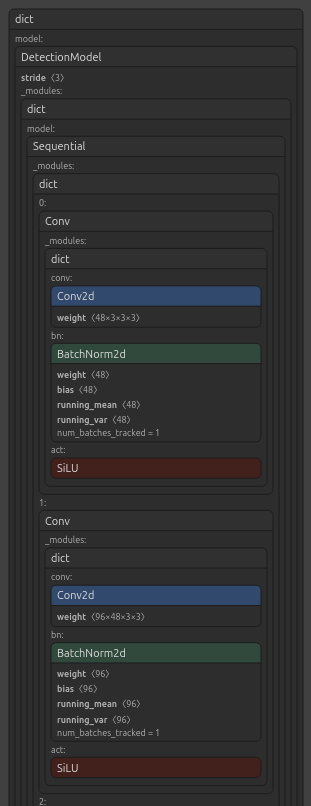
\includegraphics[width=0.37\textwidth]{images/bt4/netron_pt.png} &
        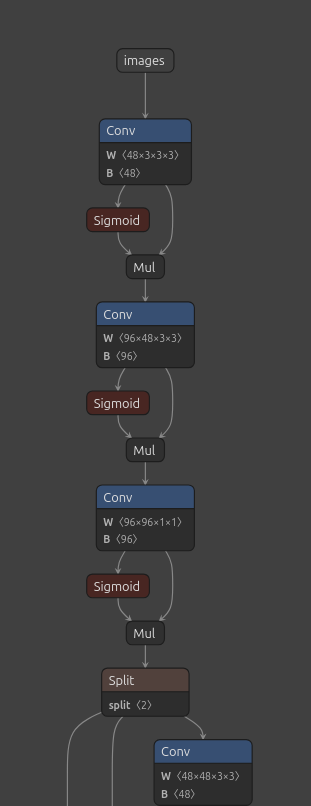
\includegraphics[width=0.37\textwidth]{images/bt4/netron_onnx.png} \\
        (a) Arquitectura .pt & (b) Arquitectura .onnx \\
    \end{tabular}
    \caption{Comparativa de arquitecturas.}
    \label{fig:qualitative_comparison}
\end{figure}

Mientras que el modelo original encapsula las operaciones complejas en módulos específicos de PyTorch de 
alto nivel como \texttt{Conv2d}, \texttt{BatchNorm2d} y \texttt{SiLU}, el modelo ONNX descompone estas operaciones en
operaciones más básicas como \texttt{Conv}, \texttt{Sigmoid} y \texttt{Mul}.
Como se observa en la Figura \ref{fig:qualitative_comparison}, las capas convolucionales se representan 
explícitamente como una secuencia de nodos, revelando la estructura a bajo nivel. La figura \ref{fig:onnx_runtime}
muestra la convergencia  de las distintas ramas de la pirámide de características. 
Se aprecian operaciones de \texttt{Reshape}, \texttt{Transpose} y \texttt{Concat} 
necesarias para unificar las predicciones a diferentes escalas en un único tensor de salida \texttt{output0}.

\begin{figure}[H]
    \centering
    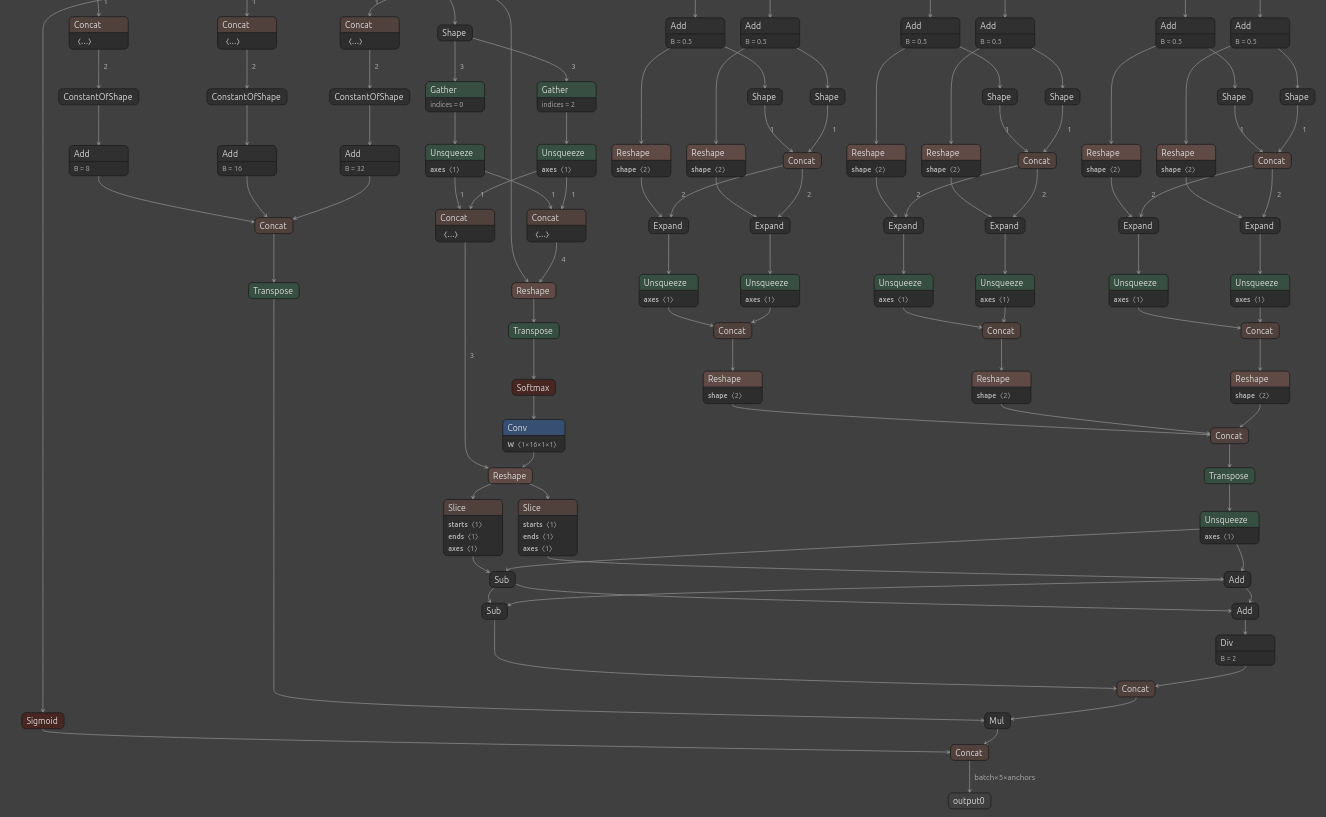
\includegraphics[width=0.9\textwidth]{images/bt4/netron_onnx2.png}
    \caption{Final del modelo YOLOv8 Medium exportado a ONNX.}
    \label{fig:onnx_runtime}
\end{figure}

Hemos verificado la equivalencia de las predicciones entre ambos formatos
utilizando una imagen de prueba. Al comparar los tensores de 
salida, la discrepancia máxima observada entre las coordenadas de las cajas 
fue de $6\times10^{-8}$ píxeles. Además, el número de detecciones fueron idénticas.
Esto confirma que la exportación a ONNX mantiene la integridad del modelo y sus capacidades predictivas,
siendo la diferencia prácticamente despreciable y atribuible 
a pequeñas variaciones numéricas inherentes a la representación en coma flotante.

\clearpage

\section*{Uso de IA}

Se ha utilizado IA conversacional para asistencia en la elaboración de código y en la comprensión de los algoritmos. Todo el contenido generado fue revisado y adaptado por los autores.

% \bibliographystyle{ieeetr}
% \bibliography{references}

\end{document}